\documentclass[a4paper]{llncs}

\usepackage{times,verbatim} % Please do not comment this
% Psfig/TeX 
\def\PsfigVersion{1.10}
\def\setDriver{\DvipsDriver} % \DvipsDriver or \OzTeXDriver
%
% All software, documentation, and related files in this distribution of
% psfig/tex are Copyright 1993 Trevor J. Darrell
%
% Permission is granted for use and non-profit distribution of psfig/tex 
% providing that this notice is clearly maintained. The right to
% distribute any portion of psfig/tex for profit or as part of any commercial
% product is specifically reserved for the author(s) of that portion.
%
% To use with LaTeX, use \documentstyle[psfig,...]{...}
% To use with TeX, use \input psfig.sty
%
% Bugs and improvements to trevor@media.mit.edu.
%
% Thanks to Ned Batchelder, Greg Hager (GDH), J. Daniel Smith (JDS),
% Tom Rokicki (TR), Robert Russell (RR), George V. Reilly (GVR),
% Ken McGlothlen (KHC), Baron Grey (BG), Gerhard Tobermann (GT).
% and all others who have contributed code and comments to this project!
%
% ======================================================================
% Modification History:
%
%  9 Oct 1990   JDS	used more robust bbox reading code from Tom Rokicki
% 29 Mar 1991   JDS	implemented rotation= option
% 25 Jun 1991   RR	if bb specified on cmd line don't check
%			for .ps file.
%  3 Jul 1991	JDS	check if file already read in once
%  4 Sep 1991	JDS	fixed incorrect computation of rotated
%			bounding box
% 25 Sep 1991	GVR	expanded synopsis of \psfig
% 14 Oct 1991	JDS	\fbox code from LaTeX so \psdraft works with TeX
%			changed \typeout to \ps@typeout
% 17 Oct 1991	JDS	added \psscalefirst and \psrotatefirst
% 23 Jun 1993   KHC     ``doclip'' must appear before ``rotate''
% 27 Oct 1993   TJD	removed printing of filename to avoid 
%			underscore problems. changed \frame to \fbox.
%			Added OzTeX support from BG. Added new
%			figure search path code from GT.
%
% ======================================================================
%
% Command synopsis:
%
% \psdraft	draws an outline box, but doesn't include the figure
%		in the DVI file.  Useful for previewing.
%
% \psfull	includes the figure in the DVI file (default).
%
% \psscalefirst width= or height= specifies the size of the figure
% 		before rotation.
% \psrotatefirst (default) width= or height= specifies the size of the
% 		 figure after rotation.  Asymetric figures will
% 		 appear to shrink.
%
% \psfigurepath{dir:dir:...}  sets the path to search for the figure
%
% \psfig
% usage: \psfig{file=, figure=, height=, width=,
%			bbllx=, bblly=, bburx=, bbury=,
%			rheight=, rwidth=, clip=, angle=, silent=}
%
%	"file" is the filename.  If no path name is specified and the
%		file is not found in the current directory,
%		it will be looked for in directory \psfigurepath.
%	"figure" is a synonym for "file".
%	By default, the width and height of the figure are taken from
%		the BoundingBox of the figure.
%	If "width" is specified, the figure is scaled so that it has
%		the specified width.  Its height changes proportionately.
%	If "height" is specified, the figure is scaled so that it has
%		the specified height.  Its width changes proportionately.
%	If both "width" and "height" are specified, the figure is scaled
%		anamorphically.
%	"bbllx", "bblly", "bburx", and "bbury" control the PostScript
%		BoundingBox.  If these four values are specified
%               *before* the "file" option, the PSFIG will not try to
%               open the PostScript file.
%	"rheight" and "rwidth" are the reserved height and width
%		of the figure, i.e., how big TeX actually thinks
%		the figure is.  They default to "width" and "height".
%	The "clip" option ensures that no portion of the figure will
%		appear outside its BoundingBox.  "clip=" is a switch and
%		takes no value, but the `=' must be present.
%	The "angle" option specifies the angle of rotation (degrees, ccw).
%	The "silent" option makes \psfig work silently.
%
% ======================================================================
% check to see if macros already loaded in (maybe some other file says
% "\input psfig") ...
\ifx\undefined\psfig\else\endinput\fi
%
% from a suggestion by eijkhout@csrd.uiuc.edu to allow
% loading as a style file. Changed to avoid problems
% with amstex per suggestion by jbence@math.ucla.edu

\let\LaTeXAtSign=\@
\let\@=\relax
\edef\psfigRestoreAt{\catcode`\@=\number\catcode`@\relax}
%\edef\psfigRestoreAt{\catcode`@=\number\catcode`@\relax}
\catcode`\@=11\relax
\newwrite\@unused
\def\ps@typeout#1{{\let\protect\string\immediate\write\@unused{#1}}}

\def\DvipsDriver{
	\ps@typeout{psfig/tex \PsfigVersion -dvips}
\def\PsfigSpecials{\DvipsSpecials} 	\def\ps@dir{/}
\def\ps@predir{} }
\def\OzTeXDriver{
	\ps@typeout{psfig/tex \PsfigVersion -oztex}
	\def\PsfigSpecials{\OzTeXSpecials}
	\def\ps@dir{:}
	\def\ps@predir{:}
	\catcode`\^^J=5
}

%% Here's how you define your figure path.  Should be set up with null
%% default and a user useable definition.

\def\figurepath{./:}
\def\psfigurepath#1{\edef\figurepath{#1:}}

%%% inserted for Searching Unixpaths
%%% (the path must end with :)
%%% (call: \DoPaths\figurepath )
%%%------------------------------------------------------
\def\DoPaths#1{\expandafter\EachPath#1\stoplist}
%
\def\leer{}
\def\EachPath#1:#2\stoplist{% #1 part of the list (delimiter :)
  \ExistsFile{#1}{\SearchedFile}
  \ifx#2\leer
  \else
    \expandafter\EachPath#2\stoplist
  \fi}
%
% exists the file (does not work for directories!)
%
\def\ps@dir{/}
\def\ExistsFile#1#2{%
   \openin1=\ps@predir#1\ps@dir#2
   \ifeof1
       \closein1
       %\ps@typeout{...not: \ps@predir#1\ps@dir#2}
   \else
       \closein1
       %\ps@typeout{...in:  \ps@predir#1\ps@dir#2}
        \ifx\ps@founddir\leer
          %\ps@typeout{set founddir #1}
           \edef\ps@founddir{#1}
        \fi
   \fi}
%------------------------------------------------------
%
% Get dir in path or error
%
\def\get@dir#1{%
  \def\ps@founddir{}
  \def\SearchedFile{#1}
  \DoPaths\figurepath
%  \fi
}
%------------------------------------------------------
%%% END of Searching Unixpaths


%
% @psdo control structure -- similar to Latex @for.
% I redefined these with different names so that psfig can
% be used with TeX as well as LaTeX, and so that it will not 
% be vunerable to future changes in LaTeX's internal
% control structure,
%
\def\@nnil{\@nil}
\def\@empty{}
\def\@psdonoop#1\@@#2#3{}
\def\@psdo#1:=#2\do#3{\edef\@psdotmp{#2}\ifx\@psdotmp\@empty \else
    \expandafter\@psdoloop#2,\@nil,\@nil\@@#1{#3}\fi}
\def\@psdoloop#1,#2,#3\@@#4#5{\def#4{#1}\ifx #4\@nnil \else
       #5\def#4{#2}\ifx #4\@nnil \else#5\@ipsdoloop #3\@@#4{#5}\fi\fi}
\def\@ipsdoloop#1,#2\@@#3#4{\def#3{#1}\ifx #3\@nnil 
       \let\@nextwhile=\@psdonoop \else
      #4\relax\let\@nextwhile=\@ipsdoloop\fi\@nextwhile#2\@@#3{#4}}
\def\@tpsdo#1:=#2\do#3{\xdef\@psdotmp{#2}\ifx\@psdotmp\@empty \else
    \@tpsdoloop#2\@nil\@nil\@@#1{#3}\fi}
\def\@tpsdoloop#1#2\@@#3#4{\def#3{#1}\ifx #3\@nnil 
       \let\@nextwhile=\@psdonoop \else
      #4\relax\let\@nextwhile=\@tpsdoloop\fi\@nextwhile#2\@@#3{#4}}
% 
% \fbox is defined in latex.tex; so if \fbox is undefined, assume that
% we are not in LaTeX.
% Perhaps this could be done better???
\ifx\undefined\fbox
% \fbox code from modified slightly from LaTeX
\newdimen\fboxrule
\newdimen\fboxsep
\newdimen\ps@tempdima
\newbox\ps@tempboxa
\fboxsep = 3pt
\fboxrule = .4pt
\long\def\fbox#1{\leavevmode\setbox\ps@tempboxa\hbox{#1}\ps@tempdima\fboxrule
    \advance\ps@tempdima \fboxsep \advance\ps@tempdima \dp\ps@tempboxa
   \hbox{\lower \ps@tempdima\hbox
  {\vbox{\hrule height \fboxrule
          \hbox{\vrule width \fboxrule \hskip\fboxsep
          \vbox{\vskip\fboxsep \box\ps@tempboxa\vskip\fboxsep}\hskip 
                 \fboxsep\vrule width \fboxrule}
                 \hrule height \fboxrule}}}}
\fi
%
%%%%%%%%%%%%%%%%%%%%%%%%%%%%%%%%%%%%%%%%%%%%%%%%%%%%%%%%%%%%%%%%%%%
% file reading stuff from epsf.tex
%   EPSF.TEX macro file:
%   Written by Tomas Rokicki of Radical Eye Software, 29 Mar 1989.
%   Revised by Don Knuth, 3 Jan 1990.
%   Revised by Tomas Rokicki to accept bounding boxes with no
%      space after the colon, 18 Jul 1990.
%   Portions modified/removed for use in PSFIG package by
%      J. Daniel Smith, 9 October 1990.
%
\newread\ps@stream
\newif\ifnot@eof       % continue looking for the bounding box?
\newif\if@noisy        % report what you're making?
\newif\if@atend        % %%BoundingBox: has (at end) specification
\newif\if@psfile       % does this look like a PostScript file?
%
% PostScript files should start with `%!'
%
{\catcode`\%=12\global\gdef\epsf@start{%!}}
\def\epsf@PS{PS}
%
\def\epsf@getbb#1{%
%
%   The first thing we need to do is to open the
%   PostScript file, if possible.
%
\openin\ps@stream=\ps@predir#1
\ifeof\ps@stream\ps@typeout{Error, File #1 not found}\else
%
%   Okay, we got it. Now we'll scan lines until we find one that doesn't
%   start with %. We're looking for the bounding box comment.
%
   {\not@eoftrue \chardef\other=12
    \def\do##1{\catcode`##1=\other}\dospecials \catcode`\ =10
    \loop
       \if@psfile
	  \read\ps@stream to \epsf@fileline
       \else{
	  \obeyspaces
          \read\ps@stream to \epsf@tmp\global\let\epsf@fileline\epsf@tmp}
       \fi
       \ifeof\ps@stream\not@eoffalse\else
%
%   Check the first line for `%!'.  Issue a warning message if its not
%   there, since the file might not be a PostScript file.
%
       \if@psfile\else
       \expandafter\epsf@test\epsf@fileline:. \\%
       \fi
%
%   We check to see if the first character is a % sign;
%   if so, we look further and stop only if the line begins with
%   `%%BoundingBox:' and the `(atend)' specification was not found.
%   That is, the only way to stop is when the end of file is reached,
%   or a `%%BoundingBox: llx lly urx ury' line is found.
%
          \expandafter\epsf@aux\epsf@fileline:. \\%
       \fi
   \ifnot@eof\repeat
   }\closein\ps@stream\fi}%
%
% This tests if the file we are reading looks like a PostScript file.
%
\long\def\epsf@test#1#2#3:#4\\{\def\epsf@testit{#1#2}
			\ifx\epsf@testit\epsf@start\else
\ps@typeout{Warning! File does not start with `\epsf@start'.  It may not be a PostScript file.}
			\fi
			\@psfiletrue} % don't test after 1st line
%
%   We still need to define the tricky \epsf@aux macro. This requires
%   a couple of magic constants for comparison purposes.
%
{\catcode`\%=12\global\let\epsf@percent=%\global\def\epsf@bblit{%BoundingBox}}
%
%
%   So we're ready to check for `%BoundingBox:' and to grab the
%   values if they are found.  We continue searching if `(at end)'
%   was found after the `%BoundingBox:'.
%
\long\def\epsf@aux#1#2:#3\\{\ifx#1\epsf@percent
   \def\epsf@testit{#2}\ifx\epsf@testit\epsf@bblit
	\@atendfalse
        \epsf@atend #3 . \\%
	\if@atend	
	   \if@verbose{
		\ps@typeout{psfig: found `(atend)'; continuing search}
	   }\fi
        \else
        \epsf@grab #3 . . . \\%
        \not@eoffalse
        \global\no@bbfalse
        \fi
   \fi\fi}%
%
%   Here we grab the values and stuff them in the appropriate definitions.
%
\def\epsf@grab #1 #2 #3 #4 #5\\{%
   \global\def\epsf@llx{#1}\ifx\epsf@llx\empty
      \epsf@grab #2 #3 #4 #5 .\\\else
   \global\def\epsf@lly{#2}%
   \global\def\epsf@urx{#3}\global\def\epsf@ury{#4}\fi}%
%
% Determine if the stuff following the %%BoundingBox is `(atend)'
% J. Daniel Smith.  Copied from \epsf@grab above.
%
\def\epsf@atendlit{(atend)} 
\def\epsf@atend #1 #2 #3\\{%
   \def\epsf@tmp{#1}\ifx\epsf@tmp\empty
      \epsf@atend #2 #3 .\\\else
   \ifx\epsf@tmp\epsf@atendlit\@atendtrue\fi\fi}


% End of file reading stuff from epsf.tex
%%%%%%%%%%%%%%%%%%%%%%%%%%%%%%%%%%%%%%%%%%%%%%%%%%%%%%%%%%%%%%%%%%%

%%%%%%%%%%%%%%%%%%%%%%%%%%%%%%%%%%%%%%%%%%%%%%%%%%%%%%%%%%%%%%%%%%%
% trigonometry stuff from "trig.tex"
\chardef\psletter = 11 % won't conflict with \begin{letter} now...
\chardef\other = 12

\newif \ifdebug %%% turn me on to see TeX hard at work ...
\newif\ifc@mpute %%% don't need to compute some values
\c@mputetrue % but assume that we do

\let\then = \relax
\def\r@dian{pt }
\let\r@dians = \r@dian
\let\dimensionless@nit = \r@dian
\let\dimensionless@nits = \dimensionless@nit
\def\internal@nit{sp }
\let\internal@nits = \internal@nit
\newif\ifstillc@nverging
\def \Mess@ge #1{\ifdebug \then \message {#1} \fi}

{ %%% Things that need abnormal catcodes %%%
	\catcode `\@ = \psletter
	\gdef \nodimen {\expandafter \n@dimen \the \dimen}
	\gdef \term #1 #2 #3%
	       {\edef \t@ {\the #1}%%% freeze parameter 1 (count, by value)
		\edef \t@@ {\expandafter \n@dimen \the #2\r@dian}%
				   %%% freeze parameter 2 (dimen, by value)
		\t@rm {\t@} {\t@@} {#3}%
	       }
	\gdef \t@rm #1 #2 #3%
	       {{%
		\count 0 = 0
		\dimen 0 = 1 \dimensionless@nit
		\dimen 2 = #2\relax
		\Mess@ge {Calculating term #1 of \nodimen 2}%
		\loop
		\ifnum	\count 0 < #1
		\then	\advance \count 0 by 1
			\Mess@ge {Iteration \the \count 0 \space}%
			\Multiply \dimen 0 by {\dimen 2}%
			\Mess@ge {After multiplication, term = \nodimen 0}%
			\Divide \dimen 0 by {\count 0}%
			\Mess@ge {After division, term = \nodimen 0}%
		\repeat
		\Mess@ge {Final value for term #1 of 
				\nodimen 2 \space is \nodimen 0}%
		\xdef \Term {#3 = \nodimen 0 \r@dians}%
		\aftergroup \Term
	       }}
	\catcode `\p = \other
	\catcode `\t = \other
	\gdef \n@dimen #1pt{#1} %%% throw away the ``pt''
}

\def \Divide #1by #2{\divide #1 by #2} %%% just a synonym

\def \Multiply #1by #2%%% allows division of a dimen by a dimen
       {{%%% should really freeze parameter 2 (dimen, passed by value)
	\count 0 = #1\relax
	\count 2 = #2\relax
	\count 4 = 65536
	\Mess@ge {Before scaling, count 0 = \the \count 0 \space and
			count 2 = \the \count 2}%
	\ifnum	\count 0 > 32767 %%% do our best to avoid overflow
	\then	\divide \count 0 by 4
		\divide \count 4 by 4
	\else	\ifnum	\count 0 < -32767
		\then	\divide \count 0 by 4
			\divide \count 4 by 4
		\else
		\fi
	\fi
	\ifnum	\count 2 > 32767 %%% while retaining reasonable accuracy
	\then	\divide \count 2 by 4
		\divide \count 4 by 4
	\else	\ifnum	\count 2 < -32767
		\then	\divide \count 2 by 4
			\divide \count 4 by 4
		\else
		\fi
	\fi
	\multiply \count 0 by \count 2
	\divide \count 0 by \count 4
	\xdef \product {#1 = \the \count 0 \internal@nits}%
	\aftergroup \product
       }}

\def\r@duce{\ifdim\dimen0 > 90\r@dian \then   % sin(x+90) = sin(180-x)
		\multiply\dimen0 by -1
		\advance\dimen0 by 180\r@dian
		\r@duce
	    \else \ifdim\dimen0 < -90\r@dian \then  % sin(-x) = sin(360+x)
		\advance\dimen0 by 360\r@dian
		\r@duce
		\fi
	    \fi}

\def\Sine#1%
       {{%
	\dimen 0 = #1 \r@dian
	\r@duce
	\ifdim\dimen0 = -90\r@dian \then
	   \dimen4 = -1\r@dian
	   \c@mputefalse
	\fi
	\ifdim\dimen0 = 90\r@dian \then
	   \dimen4 = 1\r@dian
	   \c@mputefalse
	\fi
	\ifdim\dimen0 = 0\r@dian \then
	   \dimen4 = 0\r@dian
	   \c@mputefalse
	\fi
%
	\ifc@mpute \then
        	% convert degrees to radians
		\divide\dimen0 by 180
		\dimen0=3.141592654\dimen0
%
		\dimen 2 = 3.1415926535897963\r@dian %%% a well-known constant
		\divide\dimen 2 by 2 %%% we only deal with -pi/2 : pi/2
		\Mess@ge {Sin: calculating Sin of \nodimen 0}%
		\count 0 = 1 %%% see power-series expansion for sine
		\dimen 2 = 1 \r@dian %%% ditto
		\dimen 4 = 0 \r@dian %%% ditto
		\loop
			\ifnum	\dimen 2 = 0 %%% then we've done
			\then	\stillc@nvergingfalse 
			\else	\stillc@nvergingtrue
			\fi
			\ifstillc@nverging %%% then calculate next term
			\then	\term {\count 0} {\dimen 0} {\dimen 2}%
				\advance \count 0 by 2
				\count 2 = \count 0
				\divide \count 2 by 2
				\ifodd	\count 2 %%% signs alternate
				\then	\advance \dimen 4 by \dimen 2
				\else	\advance \dimen 4 by -\dimen 2
				\fi
		\repeat
	\fi		
			\xdef \sine {\nodimen 4}%
       }}

% Now the Cosine can be calculated easily by calling \Sine
\def\Cosine#1{\ifx\sine\UnDefined\edef\Savesine{\relax}\else
		             \edef\Savesine{\sine}\fi
	{\dimen0=#1\r@dian\advance\dimen0 by 90\r@dian
	 \Sine{\nodimen 0}
	 \xdef\cosine{\sine}
	 \xdef\sine{\Savesine}}}	      
% end of trig stuff
%%%%%%%%%%%%%%%%%%%%%%%%%%%%%%%%%%%%%%%%%%%%%%%%%%%%%%%%%%%%%%%%%%%%

\def\psdraft{
	\def\@psdraft{0}
	%\ps@typeout{draft level now is \@psdraft \space . }
}
\def\psfull{
	\def\@psdraft{100}
	%\ps@typeout{draft level now is \@psdraft \space . }
}

\psfull

\newif\if@scalefirst
\def\psscalefirst{\@scalefirsttrue}
\def\psrotatefirst{\@scalefirstfalse}
\psrotatefirst

\newif\if@draftbox
\def\psnodraftbox{
	\@draftboxfalse
}
\def\psdraftbox{
	\@draftboxtrue
}
\@draftboxtrue

\newif\if@prologfile
\newif\if@postlogfile
\def\pssilent{
	\@noisyfalse
}
\def\psnoisy{
	\@noisytrue
}
\psnoisy
%%% These are for the option list.
%%% A specification of the form a = b maps to calling \@p@@sa{b}
\newif\if@bbllx
\newif\if@bblly
\newif\if@bburx
\newif\if@bbury
\newif\if@height
\newif\if@width
\newif\if@rheight
\newif\if@rwidth
\newif\if@angle
\newif\if@clip
\newif\if@verbose
\def\@p@@sclip#1{\@cliptrue}
%
%
\newif\if@decmpr
%
\def\@p@@sfigure#1{\def\@p@sfile{null}\def\@p@sbbfile{null}\@decmprfalse
   % look directly for file (e.g. absolute path)
   \openin1=\ps@predir#1
   \ifeof1
	\closein1
	% failed, search directories for file
	\get@dir{#1}
	\ifx\ps@founddir\leer
		% failed, search directly for file.bb
		\openin1=\ps@predir#1.bb
		\ifeof1
			\closein1
			% failed, search directories for file.bb
			\get@dir{#1.bb}
			\ifx\ps@founddir\leer
				% failed, lose.
				\ps@typeout{Can't find #1 in \figurepath}
			\else
				% found file.bb in search dir
				\@decmprtrue
				\def\@p@sfile{\ps@founddir\ps@dir#1}
				\def\@p@sbbfile{\ps@founddir\ps@dir#1.bb}
			\fi
		\else
			\closein1
			%found file.bb directly
			\@decmprtrue
			\def\@p@sfile{#1}
			\def\@p@sbbfile{#1.bb}
		\fi
	\else
		% found file in search dir
		\def\@p@sfile{\ps@founddir\ps@dir#1}
		\def\@p@sbbfile{\ps@founddir\ps@dir#1}
	\fi
   \else
	% found file directly
	\closein1
	\def\@p@sfile{#1}
	\def\@p@sbbfile{#1}
   \fi
}
%
%
%
\def\@p@@sfile#1{\@p@@sfigure{#1}}
%
\def\@p@@sbbllx#1{
		%\ps@typeout{bbllx is #1}
		\@bbllxtrue
		\dimen100=#1
		\edef\@p@sbbllx{\number\dimen100}
}
\def\@p@@sbblly#1{
		%\ps@typeout{bblly is #1}
		\@bbllytrue
		\dimen100=#1
		\edef\@p@sbblly{\number\dimen100}
}
\def\@p@@sbburx#1{
		%\ps@typeout{bburx is #1}
		\@bburxtrue
		\dimen100=#1
		\edef\@p@sbburx{\number\dimen100}
}
\def\@p@@sbbury#1{
		%\ps@typeout{bbury is #1}
		\@bburytrue
		\dimen100=#1
		\edef\@p@sbbury{\number\dimen100}
}
\def\@p@@sheight#1{
		\@heighttrue
		\dimen100=#1
   		\edef\@p@sheight{\number\dimen100}
		%\ps@typeout{Height is \@p@sheight}
}
\def\@p@@swidth#1{
		%\ps@typeout{Width is #1}
		\@widthtrue
		\dimen100=#1
		\edef\@p@swidth{\number\dimen100}
}
\def\@p@@srheight#1{
		%\ps@typeout{Reserved height is #1}
		\@rheighttrue
		\dimen100=#1
		\edef\@p@srheight{\number\dimen100}
}
\def\@p@@srwidth#1{
		%\ps@typeout{Reserved width is #1}
		\@rwidthtrue
		\dimen100=#1
		\edef\@p@srwidth{\number\dimen100}
}
\def\@p@@sangle#1{
		%\ps@typeout{Rotation is #1}
		\@angletrue
%		\dimen100=#1
		\edef\@p@sangle{#1} %\number\dimen100}
}
\def\@p@@ssilent#1{ 
		\@verbosefalse
}
\def\@p@@sprolog#1{\@prologfiletrue\def\@prologfileval{#1}}
\def\@p@@spostlog#1{\@postlogfiletrue\def\@postlogfileval{#1}}
\def\@cs@name#1{\csname #1\endcsname}
\def\@setparms#1=#2,{\@cs@name{@p@@s#1}{#2}}
%
% initialize the defaults (size the size of the figure)
%
\def\ps@init@parms{
		\@bbllxfalse \@bbllyfalse
		\@bburxfalse \@bburyfalse
		\@heightfalse \@widthfalse
		\@rheightfalse \@rwidthfalse
		\def\@p@sbbllx{}\def\@p@sbblly{}
		\def\@p@sbburx{}\def\@p@sbbury{}
		\def\@p@sheight{}\def\@p@swidth{}
		\def\@p@srheight{}\def\@p@srwidth{}
		\def\@p@sangle{0}
		\def\@p@sfile{} \def\@p@sbbfile{}
		\def\@p@scost{10}
		\def\@sc{}
		\@prologfilefalse
		\@postlogfilefalse
		\@clipfalse
		\if@noisy
			\@verbosetrue
		\else
			\@verbosefalse
		\fi
}
%
% Go through the options setting things up.
%
\def\parse@ps@parms#1{
	 	\@psdo\@psfiga:=#1\do
		   {\expandafter\@setparms\@psfiga,}}
%
% Compute bb height and width
%
\newif\ifno@bb
\def\bb@missing{
	\if@verbose{
		\ps@typeout{psfig: searching \@p@sbbfile \space  for bounding box}
	}\fi
	\no@bbtrue
	\epsf@getbb{\@p@sbbfile}
        \ifno@bb \else \bb@cull\epsf@llx\epsf@lly\epsf@urx\epsf@ury\fi
}	
\def\bb@cull#1#2#3#4{
	\dimen100=#1 bp\edef\@p@sbbllx{\number\dimen100}
	\dimen100=#2 bp\edef\@p@sbblly{\number\dimen100}
	\dimen100=#3 bp\edef\@p@sbburx{\number\dimen100}
	\dimen100=#4 bp\edef\@p@sbbury{\number\dimen100}
	\no@bbfalse
}
% rotate point (#1,#2) about (0,0).
% The sine and cosine of the angle are already stored in \sine and
% \cosine.  The result is placed in (\p@intvaluex, \p@intvaluey).
\newdimen\p@intvaluex
\newdimen\p@intvaluey
\def\rotate@#1#2{{\dimen0=#1 sp\dimen1=#2 sp
%            	calculate x' = x \cos\theta - y \sin\theta
		  \global\p@intvaluex=\cosine\dimen0
		  \dimen3=\sine\dimen1
		  \global\advance\p@intvaluex by -\dimen3
% 		calculate y' = x \sin\theta + y \cos\theta
		  \global\p@intvaluey=\sine\dimen0
		  \dimen3=\cosine\dimen1
		  \global\advance\p@intvaluey by \dimen3
		  }}
\def\compute@bb{
		\no@bbfalse
		\if@bbllx \else \no@bbtrue \fi
		\if@bblly \else \no@bbtrue \fi
		\if@bburx \else \no@bbtrue \fi
		\if@bbury \else \no@bbtrue \fi
		\ifno@bb \bb@missing \fi
		\ifno@bb \ps@typeout{FATAL ERROR: no bb supplied or found}
			\no-bb-error
		\fi
		%
%\ps@typeout{BB: \@p@sbbllx, \@p@sbblly, \@p@sbburx, \@p@sbbury} 
%
% store height/width of original (unrotated) bounding box
		\count203=\@p@sbburx
		\count204=\@p@sbbury
		\advance\count203 by -\@p@sbbllx
		\advance\count204 by -\@p@sbblly
		\edef\ps@bbw{\number\count203}
		\edef\ps@bbh{\number\count204}
		%\ps@typeout{ psbbh = \ps@bbh, psbbw = \ps@bbw }
		\if@angle 
			\Sine{\@p@sangle}\Cosine{\@p@sangle}
	        	{\dimen100=\maxdimen\xdef\r@p@sbbllx{\number\dimen100}
					    \xdef\r@p@sbblly{\number\dimen100}
			                    \xdef\r@p@sbburx{-\number\dimen100}
					    \xdef\r@p@sbbury{-\number\dimen100}}
%
% Need to rotate all four points and take the X-Y extremes of the new
% points as the new bounding box.
                        \def\minmaxtest{
			   \ifnum\number\p@intvaluex<\r@p@sbbllx
			      \xdef\r@p@sbbllx{\number\p@intvaluex}\fi
			   \ifnum\number\p@intvaluex>\r@p@sbburx
			      \xdef\r@p@sbburx{\number\p@intvaluex}\fi
			   \ifnum\number\p@intvaluey<\r@p@sbblly
			      \xdef\r@p@sbblly{\number\p@intvaluey}\fi
			   \ifnum\number\p@intvaluey>\r@p@sbbury
			      \xdef\r@p@sbbury{\number\p@intvaluey}\fi
			   }
%			lower left
			\rotate@{\@p@sbbllx}{\@p@sbblly}
			\minmaxtest
%			upper left
			\rotate@{\@p@sbbllx}{\@p@sbbury}
			\minmaxtest
%			lower right
			\rotate@{\@p@sbburx}{\@p@sbblly}
			\minmaxtest
%			upper right
			\rotate@{\@p@sbburx}{\@p@sbbury}
			\minmaxtest
			\edef\@p@sbbllx{\r@p@sbbllx}\edef\@p@sbblly{\r@p@sbblly}
			\edef\@p@sbburx{\r@p@sbburx}\edef\@p@sbbury{\r@p@sbbury}
%\ps@typeout{rotated BB: \r@p@sbbllx, \r@p@sbblly, \r@p@sbburx, \r@p@sbbury}
		\fi
		\count203=\@p@sbburx
		\count204=\@p@sbbury
		\advance\count203 by -\@p@sbbllx
		\advance\count204 by -\@p@sbblly
		\edef\@bbw{\number\count203}
		\edef\@bbh{\number\count204}
		%\ps@typeout{ bbh = \@bbh, bbw = \@bbw }
}
%
% \in@hundreds performs #1 * (#2 / #3) correct to the hundreds,
%	then leaves the result in @result
%
\def\in@hundreds#1#2#3{\count240=#2 \count241=#3
		     \count100=\count240	% 100 is first digit #2/#3
		     \divide\count100 by \count241
		     \count101=\count100
		     \multiply\count101 by \count241
		     \advance\count240 by -\count101
		     \multiply\count240 by 10
		     \count101=\count240	%101 is second digit of #2/#3
		     \divide\count101 by \count241
		     \count102=\count101
		     \multiply\count102 by \count241
		     \advance\count240 by -\count102
		     \multiply\count240 by 10
		     \count102=\count240	% 102 is the third digit
		     \divide\count102 by \count241
		     \count200=#1\count205=0
		     \count201=\count200
			\multiply\count201 by \count100
		 	\advance\count205 by \count201
		     \count201=\count200
			\divide\count201 by 10
			\multiply\count201 by \count101
			\advance\count205 by \count201
			%
		     \count201=\count200
			\divide\count201 by 100
			\multiply\count201 by \count102
			\advance\count205 by \count201
			%
		     \edef\@result{\number\count205}
}
\def\compute@wfromh{
		% computing : width = height * (bbw / bbh)
		\in@hundreds{\@p@sheight}{\@bbw}{\@bbh}
		%\ps@typeout{ \@p@sheight * \@bbw / \@bbh, = \@result }
		\edef\@p@swidth{\@result}
		%\ps@typeout{w from h: width is \@p@swidth}
}
\def\compute@hfromw{
		% computing : height = width * (bbh / bbw)
	        \in@hundreds{\@p@swidth}{\@bbh}{\@bbw}
		%\ps@typeout{ \@p@swidth * \@bbh / \@bbw = \@result }
		\edef\@p@sheight{\@result}
		%\ps@typeout{h from w : height is \@p@sheight}
}
\def\compute@handw{
		\if@height 
			\if@width
			\else
				\compute@wfromh
			\fi
		\else 
			\if@width
				\compute@hfromw
			\else
				\edef\@p@sheight{\@bbh}
				\edef\@p@swidth{\@bbw}
			\fi
		\fi
}
\def\compute@resv{
		\if@rheight \else \edef\@p@srheight{\@p@sheight} \fi
		\if@rwidth \else \edef\@p@srwidth{\@p@swidth} \fi
		%\ps@typeout{rheight = \@p@srheight, rwidth = \@p@srwidth}
}
%		
% Compute any missing values
\def\compute@sizes{
	\compute@bb
	\if@scalefirst\if@angle
% at this point the bounding box has been adjsuted correctly for
% rotation.  PSFIG does all of its scaling using \@bbh and \@bbw.  If
% a width= or height= was specified along with \psscalefirst, then the
% width=/height= value needs to be adjusted to match the new (rotated)
% bounding box size (specifed in \@bbw and \@bbh).
%    \ps@bbw       width=
%    -------  =  ---------- 
%    \@bbw       new width=
% so `new width=' = (width= * \@bbw) / \ps@bbw; where \ps@bbw is the
% width of the original (unrotated) bounding box.
	\if@width
	   \in@hundreds{\@p@swidth}{\@bbw}{\ps@bbw}
	   \edef\@p@swidth{\@result}
	\fi
	\if@height
	   \in@hundreds{\@p@sheight}{\@bbh}{\ps@bbh}
	   \edef\@p@sheight{\@result}
	\fi
	\fi\fi
	\compute@handw
	\compute@resv}
%
%
%
\def\OzTeXSpecials{
	\special{empty.ps /@isp {true} def}
	\special{empty.ps \@p@swidth \space \@p@sheight \space
			\@p@sbbllx \space \@p@sbblly \space
			\@p@sbburx \space \@p@sbbury \space
			startTexFig \space }
	\if@clip{
		\if@verbose{
			\ps@typeout{(clip)}
		}\fi
		\special{empty.ps doclip \space }
	}\fi
	\if@angle{
		\if@verbose{
			\ps@typeout{(rotate)}
		}\fi
		\special {empty.ps \@p@sangle \space rotate \space} 
	}\fi
	\if@prologfile
	    \special{\@prologfileval \space } \fi
	\if@decmpr{
		\if@verbose{
			\ps@typeout{psfig: Compression not available
			in OzTeX version \space }
		}\fi
	}\else{
		\if@verbose{
			\ps@typeout{psfig: including \@p@sfile \space }
		}\fi
		\special{epsf=\@p@sfile \space }
	}\fi
	\if@postlogfile
	    \special{\@postlogfileval \space } \fi
	\special{empty.ps /@isp {false} def}
}
\def\DvipsSpecials{
	%
	\special{ps::[begin] 	\@p@swidth \space \@p@sheight \space
			\@p@sbbllx \space \@p@sbblly \space
			\@p@sbburx \space \@p@sbbury \space
			startTexFig \space }
	\if@clip{
		\if@verbose{
			\ps@typeout{(clip)}
		}\fi
		\special{ps:: doclip \space }
	}\fi
	\if@angle
		\if@verbose{
			\ps@typeout{(clip)}
		}\fi
		\special {ps:: \@p@sangle \space rotate \space} 
	\fi
	\if@prologfile
	    \special{ps: plotfile \@prologfileval \space } \fi
	\if@decmpr{
		\if@verbose{
			\ps@typeout{psfig: including \@p@sfile.Z \space }
		}\fi
		\special{ps: plotfile "`zcat \@p@sfile.Z" \space }
	}\else{
		\if@verbose{
			\ps@typeout{psfig: including \@p@sfile \space }
		}\fi
		\special{ps: plotfile \@p@sfile \space }
	}\fi
	\if@postlogfile
	    \special{ps: plotfile \@postlogfileval \space } \fi
	\special{ps::[end] endTexFig \space }
}
%
% \psfig
% usage : \psfig{file=, height=, width=, bbllx=, bblly=, bburx=, bbury=,
%			rheight=, rwidth=, clip=}
%
% "clip=" is a switch and takes no value, but the `=' must be present.
\def\psfig#1{\vbox {
	% do a zero width hard space so that a single
	% \psfig in a centering enviornment will behave nicely
	%{\setbox0=\hbox{\ }\ \hskip-\wd0}
	%
	\ps@init@parms
	\parse@ps@parms{#1}
	\compute@sizes
	%
	\ifnum\@p@scost<\@psdraft{
		\PsfigSpecials 
		% Create the vbox to reserve the space for the figure.
		\vbox to \@p@srheight sp{
		% 1/92 TJD Changed from "true sp" to "sp" for magnification.
			\hbox to \@p@srwidth sp{
				\hss
			}
		\vss
		}
	}\else{
		% draft figure, just reserve the space and print the
		% path name.
		\if@draftbox{		
			% Verbose draft: print file name in box
			% 10/93 TJD changed to fbox from frame
			\hbox{\fbox{\vbox to \@p@srheight sp{
			\vss
			\hbox to \@p@srwidth sp{ \hss 
			        % 10/93 TJD deleted to avoid ``_'' problems
				% \@p@sfile
			 \hss }
			\vss
			}}}
		}\else{
			% Non-verbose draft
			\vbox to \@p@srheight sp{
			\vss
			\hbox to \@p@srwidth sp{\hss}
			\vss
			}
		}\fi	



	}\fi
}}
\psfigRestoreAt
\setDriver
\let\@=\LaTeXAtSign





% Custom command line
\usepackage{graphicx}
\usepackage{listings}
\usepackage{morefloats}
\usepackage{multicol}
\graphicspath{{artifact/images/}}

\begin{document}

\pagestyle{empty}

\mainmatter

\title{A Framework of E-commercial Recommendation Algorithms}

\titlerunning{Hudup Framework}

\author{Loc Nguyen}

\authorrunning{Loc Nguyen}

\institute{Sunflower Soft Company,\\
736084 Ho Chi Minh, Vietnam\\
\email{ng\_phloc@yahoo.com}\\
\texttt{http://www.locnguyen.net}
}

\maketitle

\begin{abstract}
Recommendation algorithm is very important to e-commercial websites when it can provide favorite products to online customers, which results out an increase in sale revenue. I propose the infrastructure for e-commercial recommendation solutions. It is a middleware framework of e-commercial recommendation software, which supports scientists and software developers to build up their own recommendation algorithms with low cost, high achievement and fast speed. This report is a full description of proposed framework, which begins with general architectures and then concentrates on programming classes. Finally, a tutorial will help readers to comprehend the framework.

\textit{Keywords}: Recommendation Algorithm, Recommendation Server, Middleware Framework.
\end{abstract}

\section{Introduction}
\label{sec:introduction}
The product provides infrastructure for e-commercial recommendation solutions, named \textit{Hudup}. This is a middleware framework of e-commercial recommendation software, which supports scientists and software developers to build up their own recommendation solutions. The term ``recommendation solution" refers to computer algorithm that introduces online customer a list of items such as books, products, services, news papers, and fashion clothes on e-commercial websites with expectation that customer will like these recommended items. The goal of recommendation algorithm is to gain high sale revenue.

You need to develop a recommendation solution for online-sale website. You, a scientist, invent a new algorithm after researching many years. Your solution is excellent and very useful and so you are very excited but:
\begin{enumerate}
\item You cope with complicated computations when analyzing big data and there are a variety of heterogeneous models in recommendation study.
\item It is impossible for you to evaluate your algorithm according to standard metrics.
\item There is no simulation environment or simulator for you to test feasibility of your algorithm.
\end{enumerate}
The innovative product Hudup supports you to solve perfectly three difficulties above and so following are your achievements: 1) Realizing your solution is very fast and easy. 2) Evaluating your solution according to standard metrics by the best way. 3) Determining feasibility of your algorithm in real-time applications.

Hudup has another preeminent function which is to provide two optimized algorithms so that it is convenient for you to assess and compare different solutions. Hudup aims to help you, a scientist or software developer, to solve three core problems above. Hudup proposes three solution stages for developing a recommendation algorithm.
\begin{enumerate}
\item \textit{Base~stage} builds up algorithm model and data model to help you to create new software with lowest cost.
\item \textit{Evaluation~stage} builds up evaluation metrics and algorithm evaluator to help you to assess your own algorithm.
\item \textit{Simulation~stage} builds up recommendation server (simulator), which helps you to test feasibility of your algorithm.
\end{enumerate}
There are now some open source softwares similar to my product. The brief list of them is described below.

\textit{Carleton} \cite{carleton} is developed by Carleton College, Minnesota, USA. The software implements some recommendation algorithms and evaluates such algorithms based on RMSE metric. The software provides an implementation illustration of recommendation algorithms and it is not recommendation framework. However, a significant feature of Carleton is to recommend courses to student based on their school reports. The schema of programming classes in Carleton is clear.

\textit{Cofi} \cite{cofi} simply implements and evaluates some recommendation algorithms. It is not recommendation framework. However, it is written by Java language \cite{oracle2014java} and it works on various platforms. This is the strong point of Cofi.

\textit{Colfi} \cite{colfi} is developed by Professor Lukas Brozovsky, Charles University in Prague, Czech Republic. The software builds up a recommendation server for dating service. It is larger than Carleton and Cofi. Colfi implements and evaluates some collaborative filtering algorithms but there is no customization support of algorithms and evaluation metrics. Note that collaborative filtering (CF) and content-based filtering (CBF) are typical recommendation algorithms. The recommendation server is simple and aims to research purposes. However, the prominent aspect of Colfi is to support dating service via client-server interaction.

\textit{Crab} \cite{crab} is recommendation server written by programming language Python. It is developed at Muricoca Labs. The strong point of Crab is to build up a recommendation engine inside the server along with algorithm evaluation mechanism. When compared with the proposed framework, Crab does not support developers to realize their solutions through three stages such as implementation, evaluation, and simulation. The architecture of Crab is not flexible and built-in algorithms are not plentiful. Most of them are SVD algorithm and nearest-neighbor algorithms.

\textit{Duine} \cite{duine} is developed by Telematica Institute, Novay. This is really a solid recommendation framework. Its architecture is very powerful and flexible. The strong point of Duine is to improve performance of recommendation engine. When compared with the proposed framework, Duine does not support developers to realize their solutions through three stages such as implementation, evaluation, and simulation. The algorithm evaluator of Duine is not standardized and its customization is not high.

\textit{easyrec} \cite{easyrec} is developed by IntelliJ IDEA and Research Studios Austria, Forschungsgesellschaft mbH. Strong points of easyrec are convenience in use, supporting consultancy via internet, and allowing users to embed recommendation engine into a website in order to call functions of easyrec from such website. However, easyrec does not support developers to build up new algorithms. This is the drawback of easyrec.

\textit{GraphLab} \cite{graphlab} is a multi-functional toolkit which supports collaborative filtering, clustering, computer vision, graph analysis, etc. It is sponsored by Office of Naval Research, Army Research Office, DARPA and Intel. GraphLab is very large and multi-functional. This strong point also implies its drawback. Developers who get familiar with GraphLab in some researches such as computer vision and graph analysis will intend to use it for recommendation study. However, GraphLab supports recommendation research with restriction. It only implements some collaborative filtering algorithms and it is not recommendation server.

\textit{LensKit} \cite{lenskit} is developed by research group GroupLen, University of Minnesota, Twin Cities, USA. It is written by programming language Java and so it works on various platforms. The strong point of LensKit is to support developers to construct and evaluate recommendation algorithms very well. The evaluation mechanism is very sophisticated. However, LensKit does not provide developers a simulator or a server that helps developers to test their solutions in client-server environment. Although the schema of programming class library is fragmentary, LenKits takes advantages of the development environment Maven. In general, LenKits is a very good recommendation framework.

\textit{Mahout} \cite{mahout} is developed by Apache Software Foundation. It is a multi-functional toolkit which supports data mining and machine learning, in which some recommendation algorithms like nearest-neighbor algorithms are implemented. Using algorithms built in Mahout is very easy. Mahout aims to end-users instead of developers. Its strong point and drawback are very similar to the strong point and drawback of GraphLab. Mahout is essentially a multi-functional toolkit and so it does not focus on recommendation system. If you intend to develop a data mining or machine learning software, you should use Mahout. If you want to focus on recommendation system, you should use the proposed framework.

\textit{MyMedia} \cite{mymedia} is a software that recommends customers media products such as movies and pictures. The preeminent feature of MyMedia is to focus on multimedia entertainment data when implementing social network mining algorithms, recommendation algorithms, and personalization algorithms. MyMedia is a very powerful multimedia recommendation framework which aims to end-users such as multimedia entertainment companies. However, MyMedia does not support specialized mechanism of algorithm evaluation based on pre-defined metrics. MyMedia, written by modern programming language C\#, is developed by EU Framework 7 Programme Networked Media Initiative together with partners: EMIC, BT, the BBC, Technical University of Eindhoven, University of Hildesheim, Microgenesis and Novay.

\textit{MyMediaLite} \cite{mymedialite} is a small programming library which implements and evaluates recommendation algorithms. MyMediaLite is light-weight software but it implements many recommendation algorithms and evaluation metrics. Its architecture is clear. These are strong points of MyMediaLite. However, MyMediaLite does not build up recommendation server. There is no customization support of evaluation metrics. These are drawbacks of MyMediaLite. MyMediaLite is developed by developers Zeno Gantner, Steffen Rendle, Lucas Drumond, and Christoph Freudenthaler at University of Hildesheim.

\textit{recommenderlab} \cite{recommenderlab} is developed by developer Michael Hahsler and sponsored by NSF Industry/University Cooperative Research Center for Net-Centric Software \& Systems. The recommenderlab is statistical extension package of R platform, which aims to build up a recommendation infrastructure based on R platform. The preeminent feature of recommenderlab is to take advantages of excellent data-processing function built in R platform. Ability to evaluate and compare algorithms is very good. However, recommenderlab does not build up recommendation server because it is dependent on R platform. The recommenderlab is suitable to algorithm evaluation in short time and scientific researches on recommendation algorithms.

\textit{SVDFeature} \cite{svdfeature}, written by programming language C++, is developed by developers Tianqi Chen, Weinan Zhang, Qiuxia Lu, Kailong Chen, Zhao Zheng, Yong Yu. SVD is a collaborative filtering algorithm which processes huge matrix very effectively in recommendation task. SVDFeature focuses on implementing SVD algorithm by the best way. Although SVDFeature is not a recommendation server, it can process huge matrix data and speed up SVD algorithm. This is the strongest point of SVDFeature.

\textit{Vogoo} \cite{vogoo} implements and deploys recommendation algorithm on webpage written by web programming language PHP. It is very fast and convenient for developers to build up e-commercial website that supports recommendation function. Although Vogoo is simple and not a recommendation server, the strongest point of Vogoo is that its library is small and neat. If fast development has top-most priority, Vogoo is the best choice.

After surveying 14 typical products, my product is the unique and most optimal if the function to support scientists and software developers through 3 stages such as algorithm implementation, quality assessment and experiment is considered most. Moreover the architecture of product is very flexible and highly customizable. Evaluation metrics to qualify algorithms are standardized according to pre-defined templates so that it is possible for software developers to modify existing metrics and add new metrics. The trial version of Hudup product is available at http://www.locnguyen.net/st/products/hudup. Architectures relevant to Hudup framework are described in section~\ref{sec:description}.

\section{General Description}
\label{sec:description}
The product is computer software which has three main modules such as \textit{Algorithm}, \textit{Evaluator} and \textit{Recommender}. These modules correspond with solution stages such as base stage, evaluation stage and simulation stage. Figure~1 depicts the general architecture of product. As seen in figure~1, the product is constituted of following modules:
\begin{itemize}
\item \textit{Algorithm}, \textit{Evaluator} and \textit{Recommender} are main modules. \textit{Algorithm}, the most important module, defines and implements abstract model of recommendation algorithms. \textit{Algorithm} defines specifications which user-defined algorithms follow. It is possible to state that \textit{Algorithm} is the infrastructure for other modules. \textit{Evaluator} is responsible for evaluating algorithms according to built-in evaluation metrics. \textit{Evaluator} also manages these built-in metrics. \textit{Recommender} is the simulation environment called \textit{simulator} which helps users to test feasibility of their algorithms in real-time applications. Thus, \textit{Recommender} is a real recommendation server. Figures 2 and 3 depict the general sub-architectures of \textit{Evaluator} and \textit{Recommender}, respectively.
\item \textit{Plugin manager}, an auxiliary module, is responsible for discovering and managing registered recommendation algorithms.
\item \textit{Parser}, which is an auxiliary module, is responsible for processing raw data. Raw data are read and modeled as \textit{Dataset} by parser. \textit{Evaluator} module evaluates algorithms based on such \textit{Dataset}. \textit{KBase}, an abbreviation of \textit{knowledge base}, is the high-level abstract model of \textit{Dataset}. For example, if recommendation algorithm mines purchase pattern of online customers from \textit{Dataset}; such pattern is represented by \textit{KBase}.
\end{itemize}
The general sub-architecture of \textit{Evaluator} shown in figure~2 implies the evaluation scenario including following steps:
\begin{enumerate}
\item Developer implements a recommendation algorithm \textit{A} based on specifications defined by \textit{Algorithm} module.
\item Developer plugs algorithm \textit{A} into \textit{Plugin manager}.
\item Scientist requires to evaluate algorithm \textit{A} by calling \textit{Evaluator}.
\item \textit{Evaluator} discovers algorithm \textit{A} via \textit{Plugin manager}. Consequently, \textit{Evaluator} loads and feeds \textit{Dataset} or \textit{KBase} to algorithm \textit{A}. If \textit{KBase} does not exist yet, algorithm \textit{A} will create its own \textit{KBase}.
\item \textit{Evaluator} executes and evaluates algorithm \textit{A} according to built-in metrics. These metrics are managed by both metrics system and \textit{Plugin manager}. In client-server environment, \textit{Evaluator} executes remotely algorithm \textit{A} by calling \textit{Recommender} module where algorithm \textit{A} is deployed. This is the most important step which is the core of evaluation process.
\item \textit{Evaluator} sends evaluation results to scientist with note that these results are formatted according to evaluation metrics aforementioned in step 5.
\end{enumerate}
Please see subsection~\ref{subsec:evaluation-package} and section~\ref{sec:tutorial} to comprehend the evaluation scenario.

The general sub-architecture of \textit{Recommender} - a recommendation server shown in figure~3 includes five layers such as interface layer, service layer, share memory layer, transaction layer, and data layer. These layers are described in bottom-up order.

\textit{Data layer} is responsible for manipulating recommendation data organized into two following formats:
\begin{itemize}
\item Low-level format is structured as rating matrix whose each row consists of user ratings on items, often called raw data. Another low-level format is \textit{Dataset} which consists of rating matrix and other information such as user profile, item profile and contextual information. \textit{Dataset} can be considered as intermediate format when it is modeled as complex and independent entity. \textit{Dataset} is the most popular format.
\item High-level format contains fine-grained information and knowledge extracted from raw data and \textit{Dataset}, for example, user interests and user purchasing pattern; besides, it may have internal inference mechanism which allows us to deduce new knowledge. High-level format structure is called \textit{knowledge base} or \textit{KBase} in short. \textit{KBase} is less popular than \textit{Dataset} because it is only used by recommendation algorithms while \textit{Dataset} is exploited widely.
\end{itemize}
Within context of \textit{Recommender} module, \textit{Dataset} and \textit{KBase} are data formats and here they do not refer to programming classes and interfaces. Because data layer processes directly read and write data operators, upper layers needs invoking data layer to access database. That data operators are transparent to upper layers provides ability to modify, add and remove components inside architecture. Data layer also supports checkpoint mechanism; whenever data is crashed, data layer will perform recovery tasks based on checkpoints so as to ensure data integrity. Note, checkpoint is the time point at which data is committed to be consistent. The current version of the product does not support recovery tasks yet. Process unit of this layer, namely read or write operator, is atomic unit over whole system. Data layer interacts directly with transaction layer via receiving and processing data operator requests from transaction layer.

\textit{Transaction layer} is responsible for managing concurrence data accesses. When many clients issue concurrently requests relating to a huge of data operators, a group of data operators in the same request is packed as an operator bunch considered as a transaction; thus, there are many transactions. In other words, transaction layer splits requests into data operators, which in turn groups data operators into transactions. Transaction is process unit of this layer. Transaction layer regulates transactions so as to ensure data consistency before sending data operators request down to data layer. Transaction layer connects directly to data layer and connects to service layer via storage service.

\textit{Share memory layer} is responsible for creating snapshot and scanner according to requirement of storage service. \textit{Snapshot} or \textit{scanner} is defined as an image of piece of \textit{Dataset} and knowledge base (\textit{KBase}) at certain time point. This image is stored in share memory for fast access because it takes long time to access data and knowledge stored in hard disk. The difference between snapshot and scanner that snapshot copies whole piece of data into memory while scanner is merely a pointer to such data piece. Snapshot consumes much more memory but gives faster access. Snapshot and scanner are read-only objects because they provide only read operator. The main responsibility of share memory layer is to create snapshots and scanners and to discard them whenever they are no longer used. Recommendation service and storage service in service layer can retrieve information of \textit{Dataset} and \textit{KBase} by accessing directly to snapshot or scanner instead of interacting with transaction layer. Hence, the ultimate goal of share memory layer is to accelerate the speed of information retrieval.

\textit{Service layer} is the heart of architecture when it realizes two goals of recommendation server: giving the list of recommended items in accordance with client request and supporting users to retrieve and update database. Such two goals are implemented by two respective services: \textit{recommender service} and \textit{storage service}. These services are main components of service layer. Recommender service receives request in the interchangeable format such as JSON format from upper layer - interface layer and analyzes this request in order to understand its content (user ratings and user profile). After that recommender service applies an effective strategy into producing a list of favorite items which are sent back to interface layer in the same interchangeable format like JSON. Recommendation strategy is defined as the co-ordination of recommendation algorithms such as collaborative filtering and content-based filtering in accordance with coherent process so as to achieve the best result of recommendation. In simplest form, strategy is identified with a recommendation algorithm. Recommender service is the most complex service because it implements both algorithms and strategies and applies these strategies in accordance with concrete situation. Recommender service is the core of aforementioned \textit{Recommender} module shown in figure~1. Storage service is simpler when it has two responsibilities:
\begin{itemize}
\item Retrieving and updating directly \textit{Dataset} and \textit{KBase} by sending access request to transaction layer and receiving results returned.
\item Requiring share memory layer to create snapshot or scanner.
\end{itemize}
Because recommendation algorithms execute on memory and recommender service cannot access \textit{Dataset} and \textit{KBase}, recommender service will require snapshot (or scanner) from storage service. Storage service, in succession, requests share memory layer to create snapshot (or scanner) and receives back a reference to such snapshot (or scanner). Such reference is used by recommender service.

\textit{Interface layer} interacts with both clients (users and application) and service layer. It is the intermediate layer having two responsibilities:
\begin{itemize}
\item For clients, it receives request from users and sends back response to them.
\item For service layer, it parses and forwards user request to service layer and receives back result.
\end{itemize}
There are two kinds of client request corresponding to two goals of recommendation server:
\begin{itemize}
\item Recommendation request is that users prefer to get favorite items.
\item Access request is that users require to retrieve or update \textit{Dataset} and \textit{KBase}.
\end{itemize}
User-specified request is parsed into interchangeable format like JSON \cite{ecma2013} because it is difficult for server to understand user-specified request in plain text format. \textit{Interpreter}, the component of interface layer, does parsing function. When users specify request as text, interpreter will parses such text into JSON object which in turn is sended to service layer. The result, for example: a list of favorite items, is returned to interpreter in form of JSON object and thus, interpreter translates such JSON result into text result easy to be understood by users.

Because server supports many clients, it is more effective if deploying server on different platforms. It means that we can distribute service layer and interface layer in different sites. Site can be a personal computer, mainframe, etc. There are many scenarios of distribution, for example, many sites for service layer and one site for interface layer. Interface layer has another component - \textit{listener} component which is responsible for supporting distributed deployment. Listener which has load balancing function is called \textit{balancer}. For example, service layer is deployed on three sites and balancer is deployed on one site; whenever balancer receives user request, it looks up service sites and choose the site whose recommender service is least busy to require such recommender service to perform recommendation task. Load balancing improves system performance and supports a huge of clients. Note that it is possible for the case that balancer or listener is deployed on more than one site.

The popular recommendation scenario includes five following steps in top-down order:
\begin{enumerate}
\item User (or client application) specifies her / his request in text format. Typical client application is the \textit{Evaluator} module shown in figure~2. \textit{Interpreter} component in \textit{interface layer} parses such text into JSON format request. \textit{Listener} component in interface layer sends JSON format request to service layer. In distributed environment, \textit{balancer} is responsible for choosing optimal service layer site to send JSON request.
\item \textit{Service layer} receives JSON request from interface layer. There are two occasions:
  \begin{enumerate}
  \item Request is to get favorite items. In this case, request is passed to recommender service. Recommender service applies appropriate strategy into producing a list of favorite items. If snapshot (or scanner) necessary to recommendation algorithms is not available in \textit{share memory layer}, recommender service requires storage service to create \textit{snapshot} (or \textit{scanner}). After that, the list of favorite items is sent back to interface layer as \textit{JSON format result}.
  \item Request is to retrieve or update data such as querying item profile, querying average rating on specified item, rating an item, and modifying user profile. In this case, request is passed to storage service. If request is to update data then, an \textit{update request} is sent to transaction layer. If request is to retrieve information then \textit{storage service} looks up share memory layer to find out appropriate snapshot or scanner. If such snapshot (or scanner) does not exists nor contains requisite information then, a \textit{retrieval request} is sent to transaction layer; otherwise, in found case, requisite information is extracted from found snapshot (or scanner) and sent back to interface layer as \textit{JSON format result}.
  \end{enumerate}
\item \textit{Transaction layer} analyzes \textit{update requests} and \textit{retrieval requests} from service layer and parses them into transactions. Each transaction is a bunch of read and write operations. All low-level operations are harmonized in terms of concurrency requirement and sent to data layer later. Some access concurrency algorithms can be used according to pre-defined isolation level.
\item \textit{Data layer} processes read and write operations and sends back \textit{raw result} to transaction layer. Raw result is the piece of information stored in \textit{Dataset} and \textit{KBase}. Raw result can be output variable indicating whether or not update (write) request is processed successfully. Transaction layer collects and sends back the raw result to service layer. Service layer translates raw result into \textit{JSON format result} and sends such translated result to interface layer in succession.
\item The \textit{interpreter} component in interface layer receives and translates \textit{JSON format result} into text format result easily understandable for users.
\end{enumerate}
The separated multilayer architecture of \textit{Recommender} module allows it to work effectively and stably with high customization; especially, its use case in co-operation with \textit{Evaluator} module is very simple. Please see the section~\ref{sec:tutorial} for comprehending how to use \textit{Recommender} and \textit{Evaluator}.

The general architecture of the product shown in figure~1 is decomposed into 9 packages as follows:
\begin{enumerate}
\item \textit{Data} package is responsible for standardizing and modeling data in abstract level. \textit{Dataset} and \textit{KBase} are built in \textit{Data} package.
\item \textit{Parser} package is responsible for analyzing and processing data.
\item \textit{Algorithm} package is responsible for modeling recommendation algorithm in abstract level. \textit{Algorithm} package supports mainly \textit{Algorithm} module.
\item \textit{Evaluation} package implements built-in evaluation mechanism of the framework. It also establishes common evaluation metrics. \textit{Evaluation} package supports mainly \textit{Evaluator} module.
\item \textit{Client} package, \textit{Server} package and \textit{Listener} package provide \textit{Recommender} module (recommendation server) in client-server network with essential support of \textit{Algorithm} package.
\item \textit{Logistic} package provides computational and mathematic utilities.
\item \textit{Plugin} package manages algorithms and evaluation metrics. It supports mainly \textit{Plugin manager} module.
\end{enumerate}
In general, three main modules \textit{Algorithm}, \textit{Evaluator} and \textit{Recommender} are constituted of such 9 packages. Figure~4 depicts these packages. Each package includes many software classes constituting internal class diagrams. Section~\ref{sec:classes} will focus on these classes. Especially, the \textit{Algorithm} package provides two optimized algorithms such as collaborative filtering algorithm based on mining frequent itemsets and collaborative filtering algorithm based on Bayesian network inference.

The product helps you to build up a recommendation algorithm fast and easily. Moreover, it is very convenient for you to assess quality and feasibility of your own algorithm in real-time application. Suppose you want to set up a new collaborative filtering algorithm called \textit{Green Fall}, instead of writing big software with a huge of complicated tasks such as processing data, implementing algorithm, implementing evaluation metrics, testing algorithm, and creating simulation environment; what you need to do is to follow three steps below:
\begin{enumerate}
\item Inheriting \textit{Recommender} class in \textit{Algorithm} package and hence, implementing your idea in two methods \textit{estimate}() and \textit{recommend}() of this class. Please distinguish \textit{Recommender} class from \textit{Recommender} module.
\item Starting up the \textit{Evaluator} module so as to evaluate and compare Green Fall with other algorithms via pre-defined evaluation metrics.
\item Configuring the \textit{Recommender} module (recommendation server) in order to embed Green Fall into such service. After that starting up \textit{Recommender} so as to test the feasibility of Green Fall in real-time applications.
\end{enumerate}
Operations in such three steps are very simple; there are mainly configurations via software graphic user interface (GUI), except that you require setting up your idea by programming code lines in step~1. Because algorithm model is designed and implemented very strictly, what you program is encapsulated in two methods \textit{estimate}() and \textit{recommend}() of \textit{Recommender} class. The average time cost to build up and test an algorithm is around 2 years but it remains 1 week for you to realize your idea if you use my product. It means that the algorithm development cost decreased very much and so it only takes 1\% original expenditure. It is really exciting work.

\section{Core Classes and Interfaces}
\label{sec:classes}
As aforementioned, Hudup is constituted of three main modules \textit{Algorithm}, \textit{Evaluator}, and \textit{Recommender} which, in turn, are decomposed into 9 packages. Each package includes many programming components but there is the limited number of core classes and interfaces on which this section focuses. Although Hudup is now implemented by Java language, it is convenient to describe classes and interfaces by UML language \cite{duong2008}. As a convention, all classes, interfaces, methods and properties complying with UML standard are written in italic font. Both class and interface are drawn as rectangles.

Class and interface are denoted as \textit{Class}, \textit{Interface}, \textit{Package}::\textit{Class}, \textit{Package}:: \textit{Interface}. If package is ignored, it is known in context. Attribute is denoted as \textit{attribute} or \textit{Class}:: \textit{attribute}.

Method is denoted as \textit{method}(), \textit{method}(\textit{parameters}), \textit{Class}::\textit{method}(\textit{parameters}), or \textit{Class}::\textit{method}(\textit{parameters}):\textit{returned}. If class is ignored, it is known in context. For a short description, method's parameters ``\textit{parameters}" and returned value ``\textit{returned}" can be ignored. For example, notations ``\textit{Recommender}:: \textit{recommend} (\textit{RecommendParam}, \textit{int}): \textit{RatingVector}", ``\textit{recommend} (\textit{RecommendParam}, \textit{int}): \textit{RatingVector}", ``\textit{recommend} (\textit{RecommendParam}, \textit{int})", ``\textit{recommend}()" indicate the same method \textit{recommend}() of \textit{Recommender} class. In fact, the method has two input parameters represented by \textit{RecommendParam} class and integer number. It returns the value represented by \textit{RatingVector} class.

UML class diagram relationships commonly used in the report are dependency, association, aggregation, composition, generalization (inheritance, derivation), and realization (implementation) as shown in figure~5.

When classes and interfaces are implemented, they are called objects or components. Some relevant classes and interfaces are grouped into a diagram and one package may own many possible diagrams. Commonly, classes and interfaces are identified with objects, subject, definitions, etc. on which they model. For example, \textit{Recommender} (class) refers to recommendation algorithm. In general, core classes and interfaces of Hudup will be described according to their packages.

\subsection{Algorithm package}
\label{subsec:algorithm-package}
The most important class of \textit{Algorithm} package is \textit{Recommender} class. It is abstract model of all recommendation algorithms. \textit{Recommender} class has two most important methods which researchers must realize according to their ideas and goals, as follows:
\begin{itemize}
\item Method \textit{estimate}(\textit{RecommendParam}, \textit{int}[]):\textit{RatingVector} whose input parameters are a recommendation parameter and a set of item identifiers. Its output result is a set of predictive or estimated rating values of items specified by the second input parameter.
\item Method \textit{recommend}(\textit{RecommendParam}, \textit{int}):\textit{RatingVector} whose input parameters are a recommendation parameter and a user identifier (user id). Its output result is a list of recommended items which is provided to the user specified by the user id.
\end{itemize}
The first input parameter of both methods represented by \textit{RecommendParam} class includes user profile represented by \textit{Profile} interface, user rating vector represented by \textit{RatingVector} class, context information, etc. The output result of both methods is represented by \textit{RatingVector} in which rating values of items are predicted (estimated). Please see subsection \ref{subsec:data-parser-packages} for more details of \textit{RatingVector}. Some algorithms calls \textit{estimate}() method inside \textit{recommend}() method; in other words, \textit{recommend}() is dependent on \textit{estimate}() in some cases. \textit{Recommender} class makes recommendation task based on executing such two methods. Ideas and features of algorithm are expressed by how methods \textit{estimate}() and \textit{recommend}() are implemented. \textit{Recommender} will call its \textit{setup}(\textit{Dataset}, \textit{Object}[] \textit{params}) method if it needs to prepare \textit{Dataset} before making recommendation task.

\textit{Recommender} class realizes directly \textit{Alg} interface which represents any algorithm. \textit{Alg} provides configuration methods such as \textit{getConfig}() and \textit{createDefaultConfig}() which allow programmers to pass customization settings to a given algorithm before it runs. Every algorithm has a unique name as returned value of \textit{getName}() method of \textit{Alg}. Plugin manager discovers automatically all algorithms via their names. \textit{Alg} is the most general interface of Hudup; anything that is programmable and executable is \textit{Alg}. As a convention, \textit{Alg} is identified with any algorithm and \textit{Recommender} is identified with recommendation algorithm. Moreover, \textit{Recommender} also refers to \textit{Recommender} module, simulator, and recommendation server aforementioned in section \ref{sec:description}. Readers distinguish them according to context. The same notation implies that recommendation server is based on recommendation algorithm. In fact, recommendation algorithm is embedded in recommender service (see figures 3, 23).

\textit{Recommender} class is executed on the dataset represented by \textit{Dataset} which is the core interface of \textit{Data} package. If programmer needs to do some pre-filtering operations before \textit{Recommender} class makes recommendation task, she/he can take advantages of \textit{Recommender}::\textit{getFilterList}() method which returns a list of filters. Each filter is represented by \textit{Filter} interface. In general, \textit{Recommender} class associates closely with classes and interfaces: \textit{Dataset}, \textit{RecommendParam}, \textit{RatingVector}, \textit{Profile}, \textit{Filter}. Figure~6 shows their diagram. \textit{Dataset}, \textit{RatingVector}, and \textit{Profile} belong to \textit{Data} package, which are mentioned later.

In recommendation study, there are two common trends such as content-based filtering (CBF) and collaborative filtering (CF) and each trend has two popular approaches such as memory-based and model-based. Correspondingly, \textit{Recommender} class is derived directly by two abstract classes \textit{MemoryBasedRecommender} and \textit{ModelBasedRecommender}. The \textit{MemoryBasedRecommender} class, in turn, is inherited by two classes \textit{MemoryBasedCBF} and \textit{MemoryBasedCF}. The \textit{ModelBasedRecommender} class, in turn, is inherited by two classes \textit{ModelBasedCBF} and \textit{ModelBasedCF}. Another class, \textit{CompositeRecommender}, is also derived directly from \textit{Recommender} class. \textit{CompositeRecommender} represents recommendation strategy aforementioned in section~\ref{sec:description}. \textit{CompositeRecommender} is combination of other \textit{Recommender} algorithms in order to produce the best list of recommended items. Figure~7 expresses inheritance relationships among these classes.

Especially, \textit{ModelBasedRecommender} applies knowledge database represented by \textit{KBase} interface into performing recommendation task. In other words, \textit{KBase} provides both necessary information and inference mechanism to \textit{ModelBasedRecommender}. Ability of inference is the unique feature of \textit{KBase}. \textit{ModelBasedRecommender} is responsible for creating \textit{KBase} by calling its \textit{createKBase}() method and so, every \textit{ModelBasedRecommender} algorithm owns distinguishable \textit{KBase}. For example, if \textit{ModelBasedRecommender} algorithm uses frequent purchase pattern to make recommendation, its \textit{KBase} contains such pattern. \textit{ModelBasedRecommender} always takes advantages of \textit{KBase} whereas \textit{MemoryBasedRecommender} uses \textit{Dataset} in execution. As aforementioned in section~\ref{sec:description}, \textit{KBase} is the high-level format and \textit{Dataset} is the low-level format. \textit{KBase} is commonly created from \textit{Dataset}. In general, \textit{KBase} is a significant aspect of \textit{Algorithm} package. Followings are essential methods of \textit{KBase}:
\begin{itemize}
\item Method \textit{setConfig}(\textit{DataConfig}) is responsible for setting configurations for \textit{KBase}. These configurations are used by other methods. The typical configuration is uniform resource identifier (URI) indicating where to store \textit{KBase}, which is used by methods \textit{load}() and \textit{save}().
\item Methods \textit{load}() and \textit{save}() are used to read/write \textit{KBase} from/to storage system, respectively. Storage system can be files, database, etc.
\item Method \textit{learn}(\textit{Dataset}, \textit{Alg}) is responsible for creating \textit{KBase} from \textit{Dataset} which is the first input parameter. Because every \textit{ModelBasedRecommender} algorithm owns distinguishable \textit{KBase}, the second parameter is such algorithm. The association between \textit{ModelBasedRecommender} and \textit{KBase} is tight.
\item Methods \textit{clear}() and \textit{isEmpty}() are responsible for cleaning out \textit{KBase} and checking whether \textit{KBase} is empty or not, respectively.
\end{itemize}
Methods of \textit{ModelBasedRecommender} always using \textit{KBase} are \textit{setup}(), \textit{createKBase}(), \textit{estimate}() and \textit{recommend}(). Especially, it is mandatory that \textit{setup}() method of \textit{ModelBasedRecommender} calls method \textit{KBase}::\textit{learn}() or \textit{KBase}::\textit{load}(). Figure~8 expresses relationships among \textit{Recommender}, \textit{Dataset}, and \textit{KBase}. The association between \textit{MemoryBasedRecommender} and \textit{Dataset} indicates that all memory-based algorithms use dataset for recommendation task.

\subsection{Data and Parser packages}
\label{subsec:data-parser-packages}
\textit{Dataset} is the core interface of \textit{Data} package. \textit{Dataset} is composed of rating matrix, user profiles, item profiles, and context information. Each row in rating matrix is a user rating vector which consists of rating values given to items by a concrete user. Rating vector is represented by \textit{RatingVector} class. Within current implementation, \textit{RatingVector} contains a set of ratings. Each rating represented by \textit{Rating} class including three attributes as follows:
\begin{itemize}
\item The \textit{rating value} that a user gives on an item. This value is represented by a real number.
\item The \textit{timestamp} identifies when such user rates on such item.
\item The \textit{context information} is represented by \textit{Context} class, for example, the place where user makes a purchase, the persons with whom user makes a purchase.
\end{itemize}
Moreover, \textit{RatingVector} provides many methods to extract and update \textit{Rating} (s). Table~1 lists some methods of user \textit{RatingVector}. For example, \textit{RatingVector}::\textit{get}(\textit{int}) method returns a \textit{Rating} that user gives to an item specified by the input parameter as item identifier.

User profile is transcript of personal information: demographic information, career, etc. Item profile contains attributes of given item: name, item type, price, etc. Both user profile and item profile are represented by \textit{Profile} class.

\textit{Dataset} interface specifies a set of methods which provide easy access to rating matrix, user profiles, item profiles, context information, etc. \textit{Dataset} is used directly by \textit{MemoryBasedRecommender} class. \textit{KBase} is created based on \textit{Dataset}. \textit{KBase} is also considered as essential model which is extracted or mined from \textit{Dataset}. Some important methods of \textit{Dataset} are listed below:
\begin{itemize}
\item Methods \textit{getUserRating}(\textit{int}) and \textit{getUserProfile}(\textit{int}) retrieve user rating vector \textit{RatingVector} and user profile \textit{Profile}, respectively given user identifier. Methods \textit{getItemRating}(\textit{int}) and \textit{getItemProfile}(\textit{int}) retrieve item rating vector \textit{RatingVector} and item profile \textit{Profile}, respectively given item identifier.
\item Methods \textit{fetchUserIds}() and \textit{fetchItemIds}() allow us to get a set of user identifiers and a set of item identifiers, respectively.
\item Method \textit{profileOf(Context)} retrieves profile information of a specified context. Context will be mentioned later.
\end{itemize}
As aforementioned in section~\ref{sec:description}, two common implementations of \textit{Dataset} are snapshot and scanner. Snapshot is represented by abstract class \textit{Snapshot}, which is a piece of dataset stored in memory. Scanner is represented by abstract class \textit{Scanner}, which is a reference to a range of dataset. It is faster to retrieve data from \textit{Snapshot} but \textit{Snapshot} consumes much more memory than \textit{Scanner} does. By default implementation of \textit{Snapshot}, rating matrix and item/user profiles are stored in hash table in which each \textit{RatingVector} or \textit{Profile} is identified by an integer number called key. Given hash table, snapshot access operators like reading \textit{RatingVector} and \textit{Profile} become faster with computational complexity \textit{O}(1) and so access time is instant. \textit{Snapshot} and \textit{Scanner} support share memory layer shown in figure~3. Figure~9 expresses diagram of \textit{Dataset} and its relevant classes.

\textit{Dataset} only provides read-only operations via ``get" and ``fetch" methods. Thus, \textit{Provider} interface and its implementations support storage service in service layer to update and modify database via writing operations. \textit{Provider} interacts directly with database, which is created in data layer. Service layer and data layer are shown in figure~3. Table~2 lists some methods of \textit{Provider}. For example, \textit{Provider}::\textit{updateRating} (\textit{RatingVector}) method saves rating values that user makes on items (specified by the input parameter \textit{RatingVector}) to database.

\textit{Provider} also provides read-only accesses to database. So, in many situations, \textit{Scanner} uses \textit{Provider} to retrieve information from database because \textit{Scanner} does not store information in memory. Moreover, \textit{Provider} manipulates context information via context template manager. Context template and context template manager are represented by interfaces \textit{ContextTemplate} and \textit{CTSManager}, which will be mentioned later. Figure~9 implicates relationships among \textit{Provider}, \textit{Scanner}, and \textit{CTSManager}. 

Context is additional information relevant to users' activities, for example, time and place that a customer purchases online. Context is modeled by \textit{Context} class. It is necessary to context-aware recommendation. Concretely, context information stored in \textit{RecommendParam} is passed to \textit{Recommender}::\textit{recommend}(\textit{RecommendParam}, \textit{int}) method whenever a recommendation request is raised. Basic methods of \textit{Context} are described as follows:
\begin{itemize}
\item Method \textit{getTemplate}() returns the template of current context. Context template will be described later.
\item Method \textit{getValue}() returns the value of current context. This value can be anything and so, it is represented by \textit{ContextValue} interface.
\item Constructor \textit{Context}(\textit{ContextTemplate}, \textit{ContextValue}) creates a context from a template and a value.
\item Method \textit{canInferFrom}(\textit{Context}) indicates whether or not the current context can be inferred from the context specified by the input parameter. Method \textit{canInferTo} (\textit{Context}) indicates whether or not the current context can lead to the context specified by the input parameter. For example, current context ``8\textsuperscript{th} December 2015" implies context ``December 2015", which means that method \textit{canInferTo}(``December 2015") returns true given the current context ``8\textsuperscript{th} December 2015".
\end{itemize}
Context can be categorized into three main types in order to answer three questions ``when, where and who" as follows \cite[pp. 224-225]{ricci2011}:
\begin{itemize}
\item Time type indicates the time when user makes a purchase, for example: date, day of week, month, year.
\item Location type indicates the place where user makes a purchase, for example: shop, market, theater, coffee house.
\item Companion type indicates the persons with whom user makes a purchase, for example: alone, friends, girlfriend/boyfriend, family, co-workers.
\end{itemize}
Context type, considered as context template, is modeled by the \textit{ContextTemplate} interface whose essential methods are described as follows:
\begin{itemize}
\item Methods \textit{getName}() and \textit{setName}(\textit{String}) are used to get and set a name of context template.
\item Method \textit{canInferFrom}(\textit{ContextTemplate}) indicates whether or not the current context template can be inferred from the context template specified by the input parameter. Method \textit{canInferTo}(\textit{ContextTemplate}) indicates whether or not the current context template can lead to the context template specified by the input parameter. These methods share the same meaning to ones of \textit{Context}. For example, template ``Year" can be inferred (extracted) from template ``Date".
\end{itemize}
Contextual information is organized in two structures such as hierarchical and multi-dimensional \cite[pp. 225-228]{ricci2011}. The default implementation of \textit{ContextTemplate} interface is \textit{HierContextTemplate} class which conforms hierarchical structure. According to hierarchical structure, templates are arranged in a tree. Figure~10 shows some \textit{HierContextTemplate} (s), in which template ``Location" is the parent of templates ``Province" and ``City" which, in turn, are parents of templates ``Suburb District", ``Town", ``District", ``Small City".

A set of many \textit{ContextTemplate} (s) compose a context template schema (CTSchema) which is specified by \textit{ContextTemplateSchema} interface. Figure~10 is an example of template schema. \textit{ContextTemplateSchema} defines methods to manipulate its \textit{ContextTemplate} members, for example:
\begin{itemize}
\item Method \textit{getRoot}() returns the root template. Method \textit{addRoot}(\textit{ContextTemplate}) adds a new root template.
\item Method \textit{getTemplateByName}(\textit{String}) retrieves a \textit{ConextTemplate} given a name.
\end{itemize}
\textit{ContextTemplateSchema} is then managed by the aforementioned interface \textit{CTSManager}. Functions of \textit{CTSManager} are specified by its main methods as follows:
\begin{itemize}
\item Method \textit{setup}(\textit{DataConfig}) is responsible for initializing \textit{ContextTemplateSchema} according to configurations specified in the input parameter.
\item Method \textit{commitCTSchema}() verifies and saves \textit{ContextTemplateSchema} to database.
\item Method \textit{getCTSchema}() allows us to retrieve \textit{ContextTemplateSchema}.
\item Each \textit{Context} is always associated with a \textit{ContextTemplate} and a \textit{ContextValue}, which implies a context is a context template evaluated by a value. So a \textit{Context} is stored in database as a \textit{Profile} which contains a \textit{ContextTemplate} and a \textit{ContextValue}. For example, context ``8\textsuperscript{th} December 2015" has template ``Date" and value ``8\textsuperscript{th} December 2015" and hence, this context is stored in database as a profile with two fields ``Date, 8\textsuperscript{th} December 2015". Therefore, \textit{CTSManager} provides method \textit{profileOf}(\textit{ContextTemplate}, \textit{ContextValue}) to retrieve a \textit{Context} given input parameters: context template and context value.
\end{itemize}
Figure~11 shows diagram of interfaces and classes relevant to context information.

Now main interfaces and classes of \textit{Data} package are described. \textit{Parser} package aims to support \textit{Data} package. Concretely, \textit{Dataset} is created from database by \textit{DatasetParser} which is the core interface of \textit{Parser} package. The main method of \textit{DatasetParser} is \textit{parse}(\textit{DataConfig}):\textit{Dataset}, which takes database configurations (database type, database connection specification, etc.) as input parameter to create \textit{Dataset} from database as returned output. Following are other methods of \textit{DatasetParser}.
\begin{itemize}
\item Method \textit{getName}() returns name of \textit{DatasetParser}, for example, ``MyParser".
\item Method \textit{support}(\textit{DataDriver}) checks whether or not a given \textit{DatasetParser} supports the kind of database (CSV file, compressed file, relation database, etc.) specified by the input parameter \textit{DataDriver}.
\end{itemize}
\textit{Snapshot} and \textit{Scanner}, two common implementations of \textit{Dataset}, are parsed by \textit{SnapshotParser} and \textit{ScannerParser} which are two inherited interfaces of \textit{DatasetParser}, respectively. \textit{MovieLensParser}, an implementation of \textit{SnapshotParser}, is responsible for reading MovieLens dataset \cite{movielens}. Figure~12 shows diagram of parsers.

\textit{DatasetParser} and \textit{CTSManager} are also \textit{Alg} interfaces because they inherits from \textit{Alg}. All \textit{Alg} classes are managed and automatically discovered by plugin manager mentioned in subsection~\ref{subsec:plugin-package}. This implies developer can add more custom parsers and context template managers. So the number of them is unlimited.

\subsection{Evaluation package}
\label{subsec:evaluation-package}
\textit{Evaluator} is the core class of \textit{Evaluation} package. Please distinguish \textit{Evaluator} class from \textit{Evaluator} module aforementioned in section~\ref{sec:description} but pay attention that \textit{Evaluator} class is the heart of \textit{Evaluator} module and they are referred mutually. \textit{Evaluator} class configures and feeds \textit{Dataset} to \textit{Recommender} class because \textit{Recommender} requires \textit{Dataset} via its method \textit{Recommender}::\textit{setup}(\textit{Dataset}) before performing recommendation task. After that \textit{Evaluator} activates two main methods of \textit{Recommender}, namely \textit{Recommender}::\textit{estimate}() and \textit{Recommender}::\textit{recommend}(). As an evaluator of any recommendation algorithm, \textit{Evaluator} is the bridge between \textit{Dataset} and \textit{Recommender} and it has six roles:
\begin{enumerate}
\item It is a loader which loads and configures \textit{Dataset}.
\item It is an executor which calls methods \textit{Recommender}::\textit{estimate}() and \textit{Recommender}:: \textit{recommend}().
\item It is an analyzer which analyzes and translates the result of algorithm execution into the form of evaluation metrics. The execution result is output of method \textit{Recommender}::\textit{estimate}() or \textit{Recommender}::\textit{recommend}(). Evaluation metric is represented by \textit{Metric} interface. \textit{Metrics} class manages a list of \textit{Metric} (s).
\item It is a registry. If external applications require receiving result from \textit{Evaluator}, they need to register with it. Such applications must implement \textit{EvaluatorListener} interface. In other words, \textit{Evaluator} contains a list of \textit{EvaluatorListener} (s).
\item Whenever it finishes a call of method \textit{Recommender}::\textit{estimate}() or \textit{Recommender}:: \textit{recommend}(), it issues a so-called evaluation event and send back evaluation metrics to external applications after executing algorithm. So it is also a provider. The evaluation event is wrapped by \textit{EvaluatorEvent} class.
\item It works as a service which allows scientists to start, pause, resume, and stop the evaluation process via its methods \textit{start}(), \textit{pause}(), \textit{resume}(), and \textit{stop}(), respectively.
\end{enumerate}
\textit{Evaluator} has four most important methods:
\begin{enumerate}
\item Method \textit{evaluate}() performs main tasks of \textit{Evaluator}, which loads \textit{Dataset} and activates method \textit{Recommender}::\textit{estimate}() or \textit{Recommender}::\textit{recommend}() on such \textit{Dataset}.
\item Method \textit{analyze}() is responsible for analyzing the result returned by method \textit{Recommender}::\textit{estimate}() or \textit{Recommender}::\textit{recommend}() so as to translate such result into evaluation metric. Metrics are used to assess algorithms and they are discussed later. By default implementation, \textit{analyze}() method will simply call \textit{Metric}::\textit{recalc}() method in order to calculate such metric itself.
\item Method \textit{issue}() issues an evaluation event and sends back evaluation metrics to external applications. Method \textit{issue}() is also named \textit{fireEvaluatorEvent}().
\end{enumerate}
These method are integrated together within current implementation of \textit{Evaluator} but their purposes are kept intact. \textit{Evaluator} is associated tightly with \textit{Recommender}, \textit{Dataset}, \textit{Metrics}, and \textit{EvaluationListener}, which is shown in figure~13.

\textit{Metric} interface specifies the final result of algorithm evaluation. In other words, there are two kinds of result.
\begin{itemize}
\item Recommendation result is represented by the output of method \textit{Recommender}:: \textit{estimate}() or \textit{Recommender}::\textit{recommend}(), which is used for recommendation process.
\item Evaluation result is represented by \textit{Metric} interface which is the output of \textit{Evaluator}::\textit{analyze}(). It is derived from recommendation result and used for qualifying algorithm.
\end{itemize}
Followings are essential methods of \textit{Metric}:
\begin{itemize}
\item Method \textit{recalc}(\textit{Object}[]) is the most important one expressing how to calculate a concrete \textit{Metric}. It is called by \textit{Evaluator}::\textit{analyze}(). Its input parameter is array of objects passed by \textit{Evaluator}.
\item Methods \textit{getAccumValue}() and \textit{getCurrentValue}() return accumulative value and current value of metric. After each time \textit{Metric} is calculated by \textit{recalc}(\textit{Object}[]) method, accumulative value and current value can be changed. For example, a sample \textit{Metric} receives values 3, 1, 2 at the first, second, and third calculations. At the fourth calculation if \textit{recalc}(\textit{Object}[]) produces value 2, the \textit{getCurrentValue}() will return 2 and the \textit{getAccumValue}() will return 3 + 1 + 2 + 2 = 8. Methods \textit{getAccumValue}() and \textit{getCurrentValue}() can return any thing and so their returned value is represented by \textit{MetricValue} interface. How to implement \textit{MetricValue} is dependent on concrete application.
\end{itemize}
The abstract class of \textit{Metric} interface is \textit{AbstractMetric}. Three implemented classes of \textit{Metric} which inherit from \textit{AbstractMetric} are \textit{DefaultMetric}, \textit{MetaMetric}, and \textit{MetricWrapper} as follows:
\begin{itemize}
\item \textit{DefaultMetric} class is default implementation of single \textit{Metric}.
\item \textit{MetaMetric} class is a complex \textit{Metric} which contains other metrics.
\item In some situations, if metric requires complicated implementation, it is wrapped by \textit{MetricWrapper} class.
\end{itemize}
The \textit{Metrics} class manages a list of \textit{Metric} (s). It uses \textit{MetricWrapper} for sophisticated management tasks. Exactly, \textit{Metrics} contains \textit{MetricWrapper} objects and each such object wraps a \textit{Metric} template. Figure~14 shows diagram of metrics.

Currently, two default metrics inherited from \textit{DefaultMetric} class are \textit{TimeMetric} class and \textit{Accuracy} class. \textit{TimeMetric} measures the speed of algorithm and so it is the time in seconds that methods \textit{Recommender}::\textit{estimate}() and \textit{Recommender}::\textit{recommend}() execute over \textit{Dataset}.

\textit{Accuracy} reflects goodness and efficiency of recommendation algorithms. There are three types of accuracy.
\begin{itemize}
\item Predictive accuracy, represented by \textit{PredictiveAccuracy} class, measures how close predicted ratings returned from methods \textit{Recommender}::\textit{estimate}() and \textit{Recommender} :: \textit{recommend}() are to the true user ratings \cite[pp. 20-21]{herlocker2004}. \textit{PredictiveAccuracy} class derives directly from \textit{Accuracy} class. \textit{MAE}, \textit{MSE}, \textit{RMSE} \cite[pp. 20-21]{herlocker2004} are typical predictive accuracy metrics.
\item Classification accuracy, represented by \textit{ClassificationAccuracy} class, measures the frequency that methods \textit{Recommender}::\textit{estimate}() and \textit{Recommender}::\textit{recommend}() make correct or incorrect recommendation \cite[pp. 20-22]{herlocker2004}. \textit{ClassificationAccuracy} class derives directly from \textit{Accuracy} class. \textit{Precision} and \textit{Recall} \cite[pp. 22-25]{herlocker2004} are typical classification accuracy metrics.
\item Correlation accuracy, represented by \textit{CorrelationAccuracy} class, measures the ability that method \textit{Recommender}::\textit{recommend}() makes the ordering of recommended items which is similar to the ordering of user's favorite items \cite[pp. 29-33]{herlocker2004}. \textit{CorrelationAccuracy} class derives directly from \textit{Accuracy} class. \textit{NDPM}, \textit{Spearman}, \textit{Pearson} \cite[pp. 29-33]{herlocker2004} are typical correlation accuracy metrics.
\end{itemize}
Figure~15 lists these default metrics known as pre-defined or built-in metrics. \textit{Metric} like \textit{Algorithm}::\textit{Recommender}, \textit{Data}::\textit{CTSManager}, \textit{Parser}::\textit{DatasetParser} is also \textit{Alg} interface because it derives from \textit{Alg}. So developers can define new metrics.

If external applications want to receive metrics, they need to register with \textit{Evaluator} by calling \textit{Evaluator}::\textit{addListener}() method. The evaluation process has five steps:
\begin{enumerate}
\item \textit{Evaluator} calls \textit{Evaluator}::\textit{evaluate}() method to load and feed \textit{Dataset} to \textit{Recommender}.
\item Method \textit{Recommender}::\textit{estimate}() or \textit{Recommender}::\textit{recommend}() is executed by \textit{Evaluator}::\textit{evaluate}() method to perform recommendation task.
\item Method \textit{Evaluator}::\textit{analyze}() analyzes the result returned by method \textit{Recommender}:: \textit{estimate}() or \textit{Recommender}::\textit{recommend}() and translates such result into \textit{Metric}. The \textit{Metrics} class manages a list of \textit{Metric} (s).
\item External applications that implement \textit{EvaluatorListener} interface register with \textit{Evaluator} by calling \textit{Evaluator}::\textit{addListener}() method.
\item Method \textit{Evaluator}::issue() sends \textit{Metrics} to external applications.
\end{enumerate}
Figure~16 is a view of such five steps.

\subsection{Client, Server, and Listener packages}
\label{subsec:client-server-listener-package}
\textit{Client} package defines classes and interfaces necessary to client-server network. Following are basic classes and interfaces in \textit{Client} package:
\begin{itemize}
\item \textit{Request} class represents user request. \textit{Request} uses JSON format \cite{ecma2013} as exchangeable means in client-server network. As aforementioned in section~\ref{sec:description}, user request includes recommendation request, retrieval request, update request.
  \begin{itemize}
  \item Recommendation \textit{Request} is that user prefers to get favorite items. Exactly, this \textit{Request} wraps \textit{RecommendParam} which is the first input parameter of methods \textit{Recommender}::\textit{estimate}() and \textit{Recommender}::\textit{recommend}().
  \item Retrieval or update \textit{Request} is that user wants to retrieve or update her/his ratings and profiles.
  \end{itemize}
\item \textit{Response} class represents result of recommendation process. \textit{Response} uses JSON format as exchangeable means.
  \begin{itemize}
  \item In case of recommendation request, \textit{Response} is the list of recommended items returned from service layer (see figure~3). Exactly, \textit{Response} wraps the returned \textit{RatingVector} of methods \textit{Recommender}::\textit{estimate}() and \textit{Recommender}:: \textit{recommend}().
  \item For update request, \textit{Response} is the output variable indicating whether or not update request is successful.
  \item For retrieval request, \textit{Response} is the piece of information stored in \textit{Dataset} or \textit{KBase}. If information is stored in \textit{Dataset}, \textit{Response} often wraps a returned \textit{Snapshot}.
  \end{itemize}
\item \textit{Protocol} interface specifies methods to create \textit{Request} in many possible cases. \textit{Protocol} establishes an interaction protocol of Hudup client-server network, which is named ``hdp". Table~3 shows some methods of \textit{Protocol}.
\item \textit{Service} interface specifies methods to serve user requests. These methods focus on providing recommendation, inserting, updating and getting information such as user ratings, user profiles, and item profiles stored in database. Storage service and recommender service (see figure~3) implement \textit{Service} interface. They are typical \textit{Service} (s). Table~4 lists some methods of \textit{Service}.
\item \textit{Server} interface defines abstract model of recommendation server. \textit{Server} is responsible for creating \textit{Service} to serve user requests. \textit{Server} starts, pauses, resumes, and stops by methods \textit{start}(), \textit{pause}(), \textit{resume}(), and \textit{stop}(), respectively. It must be implemented by programmer. Both \textit{Server} and \textit{Service} constitute a proper recommendation server.
\end{itemize}
Association relationships among \textit{Request}, \textit{Response}, \textit{Protocol}, \textit{Service}, and \textit{Server} are tight. Figure~17 shows diagram of \textit{Client} package.

\textit{Server} package focuses on implementing recommendation server. Following are classes and interfaces in \textit{Server} package:
\begin{itemize}
\item \textit{DefaultService} class is default implementation of aforementioned \textit{Client}::\textit{Service} interface. \textit{DefaultService} uses \textit{Recommender} and \textit{Data}::\textit{Provider} for processing recommendation request and update request, respectively. Developers are suggested to build up their own services.

\item \textit{DefaultServer} class is default implementation of aforementioned \textit{Client}::\textit{Server} interface. \textit{DefaultServer} creates and manages \textit{DefaultService}. Developers are suggested to build up their own servers.

\item \textit{Transaction} interface represents transaction layer (see figure~3) in the architecture of \textit{Recommender} module. \textit{Transaction} is responsible for managing concurrence data accesses. Currently, \textit{DefaultServer} is responsible for implementing \textit{Transaction} interface.

\item \textit{ActiveMeasure} interface specifies how to measure the active degree of \textit{DefaultServer}. For example, there is a counter inside \textit{ActiveMeasure}. Each time \textit{DefaultServer} receives a user request, the counter is increased by 1. After \textit{DefaultServer} finishes serving such user request, the counter is decreased by 1. If there are many \textit{DefaultServer} (s) deployed on different sites, balancer aforementioned in section~\ref{sec:description} uses \textit{ActiveMeasure} to determine which \textit{DefaultServer} is least busy in order to dispatch user request to such \textit{DefaultServer} whose active counter is smallest.
\end{itemize}
Figure~18 shows diagram of \textit{Server} package.

\textit{Listener} package focuses on implementing listener and balancer aforementioned in section~\ref{sec:description}. Following are classes in \textit{Listener} package:
\begin{itemize}
\item \textit{Listener} class represents a listener shown in figure~3. \textit{Listener} also implements \textit{Client}::\textit{Server} but it is not recommendation server. \textit{Listener} is deployed in interface layer, which supports distributed environment. \textit{Listener} stores a list of binding \textit{Server}::\textit{DefaultServer} (s). It can bind a new \textit{Server}::\textit{DefaultServer} by calling its \textit{rebind}(\textit{Server}) method. In case that there are many \textit{Server}::\textit{DefaultServer} (s) and one \textit{Listener} then, \textit{Listener} is responsible for dispatching user requests to its proper binding \textit{Server}::\textit{DefaultServer}. \textit{Listener} starts, pauses, resumes, and stops by its methods \textit{start}(), \textit{pause}(), \textit{resume}(), and \textit{stop}(), respectively.

\item \textit{Delegator} class implements \textit{Client}::\textit{Protocol}, which is responsible for handling and processing user request represented by \textit{Client}::\textit{Request}. Each time \textit{Listener} receives a user request, it creates a respective \textit{Delegator} and passes such request to \textit{Delegator}. After that \textit{Delegator} processes and dispatches the request to the proper binding \textit{Server}::\textit{DefaultServer}. The result of recommendation process from \textit{Server}::\textit{DefaultServer}, represented by \textit{Client}::\textit{Response}, is sent back to users/applications by \textit{Delegator}. In fact, \textit{Delegator} interacts directly with \textit{Server}::\textit{DefaultServer}. However, \textit{Delegator} is a part of \textit{Listener} and the client-server interaction is always ensured.

\item \textit{Balancer} class represents a balancer shown in figure~3. \textit{Balancer} derives from \textit{Listener} and overrides the \textit{rebind}(\textit{Server}) method in order to support balancing function while it inherits all other functions of \textit{Listener}. \textit{Balancer} selects least busy binding \textit{Server}::\textit{DefaultServer} to which user requests are dispatched. Therefore, \textit{Balancer} improves system performance more than \textit{Listener} does. In general, \textit{Listener} and \textit{Balancer} are main components of interface layer.
\end{itemize}
Figure~19 shows diagram of \textit{Listener} package.

In general, three packages \textit{Client}, \textit{Server}, and \textit{Listener} with support of package \textit{Algorithm} compose \textit{Recommender} module - a complete recommendation server which is also called simulator.

\subsection{Plugin package}
\label{subsec:plugin-package}
\textit{PluginManager} interface and \textit{RegisterTable} class are main parts of \textit{Plugin} package. Both of them are initialized whenever Hudup framework boots. Method \textit{discover}() of \textit{PluginManager} is executed at starting time of Hudup, which automatically discovers all algorithms that implement \textit{Alg} interface and registers such algorithms in \textit{RegisterTable}. \textit{RegisterTable} then manages these algorithms. \textit{RegisterTable} provides two important methods \textit{register}(\textit{Alg}) and \textit{query}(\textit{String}) as follows:
\begin{itemize}
\item Method \textit{register}(\textit{Alg}) registers a given algorithm. This method is called by \textit{PluginManager}::\textit{discover}() at starting time of Hudup.
\item Method \textit{query}(\textit{String}) retrieves an algorithm by its name with attention that such algorithm is named by returned value of its \textit{Alg}::\textit{getName}() method. Method \textit{query} (\textit{String}) is often called by \textit{Evaluation}::\textit{Evaluator} and \textit{Client}::\textit{Service}.
\end{itemize}
\textit{Algorithm}::\textit{Recommender}, \textit{Data}::\textit{CTSManager}, \textit{Parser}::\textit{DatasetParser}, and \textit{Evaluation} ::\textit{Metric} are typical \textit{Alg} (s), managed by \textit{RegisterTable}. This implies \textit{Plugin} package supports the high customization of Hudup. Scientists and software developers can define any algorithm following \textit{Alg} specifications and put such algorithm in Hudup framework (Hudup class path). Consequently, \textit{PluginManager} discovers the algorithm automatically and \textit{RegisterTable} stores it for later use. It is easy for \textit{Evaluation}::\textit{Evaluator} and \textit{Client}::\textit{Service} to get the user-defined algorithm by calling \textit{RegisterTable}::\textit{query} (\textit{String}). \textit{Plugin} package is small but it is very important for Hudup framework. Figure~20 shows diagram of \textit{Plugin} package.

Core components of Hudup, classes and interfaces, are now described in details so that readers can comprehend the Hudup infrastructure. Section~\ref{sec:tutorial} is a tutorial on how to use Hudup product.

\section{Tutorial on Proposed Framework}
\label{sec:tutorial}
Suppose you want to set up Green Fall algorithm - a collaborative filtering algorithm based on mining frequent itemsets. You save a lot of efforts and resources when taking advantages of the proposed framework. This tutorial has three simple steps to implement, evaluate, and deploy your custom algorithm, corresponding to three stages aforementioned in section \ref{sec:introduction} such as base stage, evaluation stage, and simulation stage. These steps are explained in subsections \ref{subsec:tutorial-implementing}, \ref{subsec:tutorial-evaluating}, and \ref{subsec:tutorial-deploying}, respectively. 

\subsection{Implementing algorithm}
\label{subsec:tutorial-implementing}
Firstly, you create the Java project named Green Fall and import the core Java library package ``hudup-core.jar" into Green Fall project; the core library contains all core classes and interfaces aforementioned in section~\ref{sec:classes}. This starts the base stage proposed by Hudup framework. Note that Hudup is written by the object-oriented language Java \cite{oracle2014java}. You create the \textit{GreenFall} class inheriting from \textit{ModelBasedCF} class because Green Fall is model-based recommendation algorithm. Before implementing your idea in two methods \textit{estimate}() and \textit{recommend}() of \textit{GreenFall}, you create its knowledge base \textit{GreenFallKB} derived directly from \textit{KBase}. \textit{GreenFallKB} will contains frequent itemsets. Following is abstract code of \textit{GreenFallKB} class in which you must override the \textit{GreenFallKB}::\textit{learn}() method to mine frequent itemsets from \textit{Dataset}, according to code lines 5-7:
\begin{small}
\begin{lstlisting}[language=Java]
(01) class GreenFallKB implements KBase {
(02)   ...
(03)   Itemsets frequentItemsets;
(04)
(05)   public void learn(Dataset dataset, Alg alg) {
(06)     //Your code hear to mine frequent itemsets
(07)   }
(08)
(09)   Itemsets getFrequentItemsets() {return frequentItemsets;}
(10)   ...
(11) }
\end{lstlisting}
\end{small}
Your idea is realized in methods \textit{estimate}() and \textit{recommend}() of main class \textit{GreenFall} as follows:
\begin{small}
\begin{lstlisting}[language = Java]
(01) public class GreenFall extends ModelBasedCF {
(02)   ...
(03)   GreenFallKB kb;
(04)
(05)   public String getName() {return "gfall";}
(06)
(07)   public void setup(Dataset dataset) {
(08)     kb = new GreenFallKB();
(09)     kb.learn(dataset, this);
(10)   }
(11)
(12)   public RatingVector estimate(RecommendParam param,
(13)       int[] itemIds) {
(14)     Itemsets frequentItemsets = kb.getFrequentItemsets();
(15) 
(16)     RatingVector vEstimated=null;
(17)     //Your code here to estimate missing values
(18)     //based on frequent itemsets
(19)
(20)     return vEstimate;
(21)   }
(22)
(23)   public RatingVector recommend(RecommendParam param,
(24)       int userId) {
(25)     Itemsets frequentItemsets = kb.getFrequentItemsets();
(26)
(27)     RatingVector vRecommended = null;
(28)     //Your code here to produce recommended items
(29)     //based on frequent itemsets
(30)
(31)     return vRecommended;
(32)   }
(33)   ...
(34) }
\end{lstlisting}
\end{small}
According to the code lines 12-21 and 23-32 above, methods \textit{GreenFall}::\textit{estimate}() and \textit{GreenFall}::\textit{recommend}() apply frequent itemsets resulted from \textit{GreenFallKB} into estimating rating values of given items and producing recommended items of given user, respectively. All things you do manually are to implement these two methods. The short name of Green Fall algorithm is ``gfall" as the returned value of \textit{getName}() method (see code line 5). Now you compile the Green Fall project and compress it into the Java package ``gfall.jar". Subsequently, you put the package ``gfall.jar" into library directory of Hudup so that \textit{PluginManager} can discover and register Green Fall algorithm in \textit{RegisterTable}.

\subsection{Evaluating algorithm}
\label{subsec:tutorial-evaluating}
Secondly, you open \textit{Evaluator} to assess Green Fall algorithm, as shown in figure~21. This is evaluation stage proposed by Hudup framework. Exactly, what you see in figure~21 is the graphic user interface (GUI) of \textit{Evaluator} module. As a convention, this GUI refers to \textit{Evaluator} in the tutorial.

The \textit{Evaluator} discovers the Green Fall algorithm via the name ``gfall". Exactly, \textit{Evaluator} calls \textit{RegisterTable}::\textit{query}(``gfall") to retrieve it. Now you evaluate the Green Fall algorithm by \textit{Evaluator}. Database Movielens \cite{movielens} is used for evaluation but you do not need to focus on its structure because \textit{Evaluator} processes it automatically. Moreover, the complex evaluation mechanism and metrics system built in \textit{Evaluator} are automatically applied into evaluating Green Fall algorithm according to pre-defined metrics. Four important pre-defined metrics aforementioned in subsection \ref{subsec:evaluation-package} are used in this evaluation: \textit{MAE}, \textit{Precision}, \textit{Recall}, and \textit{TimeMetric}. \textit{TimeMetric} known as speed metric is calculated in seconds. \textit{MAE} is predictive accuracy metric that measures how close predicted value is to rating value. The less \textit{MAE} is, the high accuracy is. \textit{Precision} and \textit{Recall} are quality metrics that measure the quality of recommendation list – how much the recommendation list reflects user's preferences. The large quality metric is, the better algorithm is.

\textit{Evaluator} allows you to define custom metrics. Suppose we create a new metric called \textit{MSE} which is a predictive accuracy metric. \textit{MSE}, abbreviation of mean squared error, measures the average squared deviation between the predictive rating and user's true rating \cite{herlocker2004}. Note that methods \textit{Recommender}::\textit{estimate}() and \textit{Recommender}:: \textit{recommend}() return predictive (estimated) ratings. \textit{MSE} is calculated by equation (\ref{math:mse}).
\begin{equation} \label{math:mse}
MSE = \frac{\sum_{i=1}^{n}(p_i-v_i)^2}{n}
\end{equation}
Where $n$ is the total number of recommended items while $p_i$ and $v_i$ are predictive rating and true rating of item $i$, respectively. In order to realize equation (\ref{math:mse}), you create the new \textit{MSE} class derived from \textit{PredictiveAccuracy} class and override \textit{calc}() method, as follows:
\begin{small}
\begin{lstlisting}[language = Java]
(01) public class MSE extends PredictiveAccuracy {
(02)   ...
(03)   public String getName() {return "MSE";}
(04)
(05)   protected MetricValue calc(RatingVector vPredicted,
(06)     RatingVector vTrue) {
(07) 
(08)     float sum = 0;
(09)     int n = 0;
(10)     int[] itemIds = vPredicted.getItemIds();
(11)     for (int itemId : itemIds) {
(12)       float dev=vPredicted.get(itemId)-vTrue.get(itemId));
(13)       sum += dev * dev;
(14)       n++;
(15)     }
(16) 
(17)     return new FractionMetricValue(sum, n);
(18)   }
(19)   ...
(20) }
\end{lstlisting}
\end{small}
The \textit{calc}() will be called by the \textit{Metric}::\textit{recalc}() which, in turn, is called by the \textit{Evaluator}::\textit{analyze}(). According to code lines 5-6, \textit{vPredicted} and \textit{vTrue} represent predictive ratings and user's true ratings. At lines 8-15, the sum $\sum_{i=1}^{n}(p_i-v_i)^2$ inside equation (\ref{math:mse}) is calculated. At line 17, specific \textit{FractionMetricValue} representing the value of \textit{MSE} is returned. \textit{FractionMetricValue} class with two atributes $a$ and $b$, an implementation of \textit{MetricValue} interface, represents a fraction in form of $\frac{a}{b}$. \textit{MSE} metric is an \textit{Alg} and so its name ``MSE" is returned value of the \textit{getName}() method at line 3 so that it is registered by \textit{PluginManager}.

Now you put \textit{MSE} class into package ``gfal.jar" so that \textit{Evaluator} can discover it. Consequently, you execute \textit{Evaluator} to evaluate Green Fall algorithm according to five metrics: \textit{MAE}, \textit{MSE}, \textit{Precision}, \textit{Recall}, and \textit{TimeMetric}. Figure~22 shows the evaluation result in which the speed of Green Fall algorithm is 0.0055. Currently, iconic images of GUI (s) shown in figures 21, 22, 23, 24, 25, 26 are used temporarily and so they will be designed particularly.

\subsection{Deploying algorithm}
\label{subsec:tutorial-deploying}
Finally, \textit{Recommender} module, a recommendation server, supports you to deploy and test Green Fall algorithm in real-time application. This is simulation stage proposed by Hudup framework. When you put the package ``gfall.jar" into library directory of Hudup, \textit{Recommender} automatically discovers and deploys Green Fall on server, as seen in figure~23. Moreover, \textit{Recommender} allows you to configure Green Fall for particular purposes. \textit{Recommender} serves client requests at server port 10151.

You start up and configure \textit{Listener} to connect with \textit{Recommender}. As seen in figure~24, \textit{Listener} connects with \textit{Recommender} through server port 10151 and it serves client requests at listener port 10152.
Consequently, you configure \textit{Evaluator} to connect with \textit{Listener}. As seen in figure~25, \textit{Evaluator} connects successfully with \textit{Listener} through listener port 10152. The connection between \textit{Evaluator} and \textit{Listener} complies with the basic socket protocol. Now \textit{Listener} becomes a bridge between \textit{Evaluator} and Recommender, which allows \textit{Evaluator} to call Green Fall algorithm deployed remotely in \textit{Recommender}.

Now you use \textit{Evaluator} to test Green Fall algorithm via client-server environment with cooperation of \textit{Evaluator}, \textit{Listener}, and \textit{Recommender}. Figure~26 shows again the evaluation result of Green Fall algorithm from remote execution. \textit{Evaluator} interacts with \textit{Listener} through listener port 10152 and \textit{Listener}, in turn, interacts with \textit{Recommender} through server port 10151. Due to network transportation, the speed of Green Fall algorithm is decreased, which is 0.0347 whereas it is 0.0055 given local execution as seen in figure~22. However, the decrease of speed is insignificant within two cases as follows:
\begin{itemize}
\item \textit{Recommender} server is deployed on a powerful computer. Cost of network transportation is smaller than cost of algorithm execution.
\item There are many \textit{Recommender} servers deployed in distributed environment and \textit{Listener} is replaced by \textit{Balancer} which supports balancing mechanism aforementioned in subsection \ref{subsec:client-server-listener-package}.
\end{itemize}

\begin{figure}
\centering
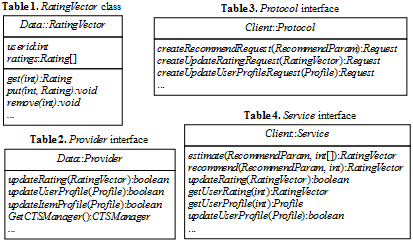
\includegraphics{MultiTables.png}
\end{figure}

\begin{figure}
\centering
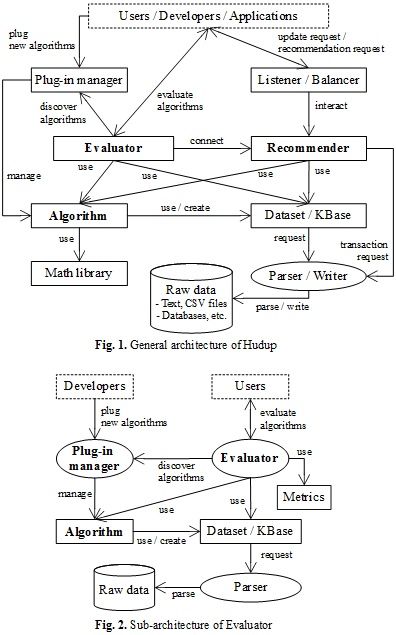
\includegraphics{MultiFigures-1.png}
\end{figure}

\begin{figure}
\centering
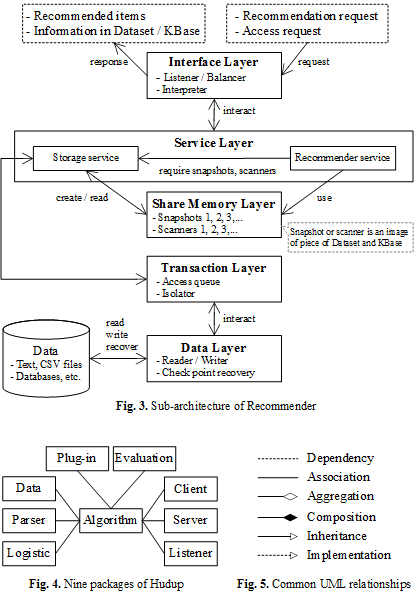
\includegraphics{MultiFigures-2.png}
\end{figure}

\begin{figure}
\centering
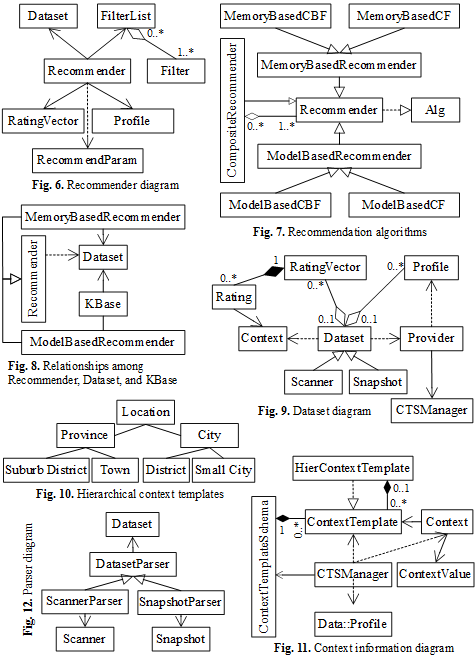
\includegraphics{MultiFigures-3.png}
\end{figure}

\begin{figure}
\centering
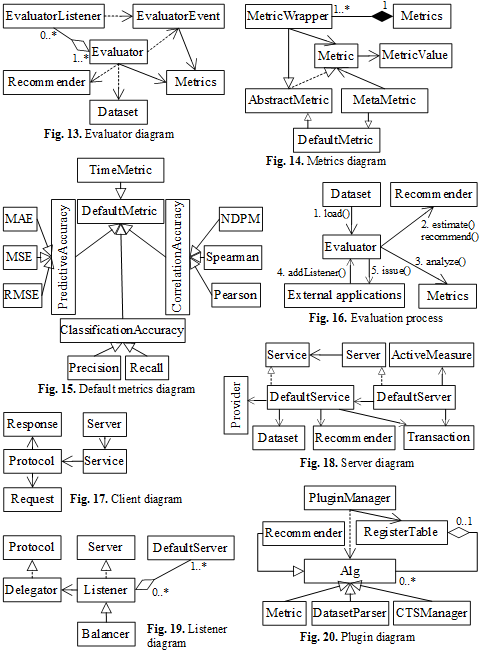
\includegraphics{MultiFigures-4.png}
\end{figure}

\begin{figure}
\centering
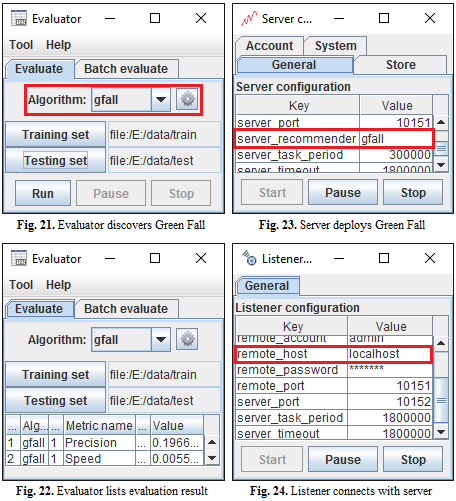
\includegraphics{MultiFigures-5.png}
\end{figure}

\begin{figure}
\centering
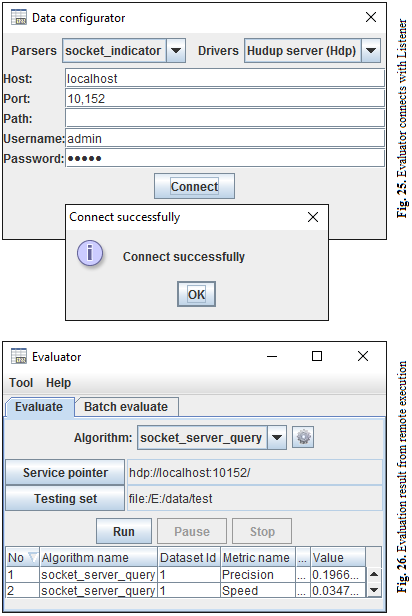
\includegraphics{MultiFigures-6.png}
\end{figure}

\section{Conclusions}
\label{sec:conclusions}
In general, it is easy for you to implement, evaluate and deploy your solution by taking advantages of the proposed framework. Most tasks are configured via friendly GUI. Complicated operations are processed by services and you only focus on realizing your ideas. Hudup, a framework of e-commercial recommendation algorithms, is the best choice for you to build up a recommendation solution. Moreover, it is not only used for e-commercial software but also applied into any application in which recommendation is necessary.

The framework has 6 most essential components (classes and interfaces) such as \textit{Algorithm}::\textit{Recommender}, \textit{Data}::\textit{Dataset}, \textit{Data}::\textit{KBase}, \textit{Evaluation}::\textit{Evaluator}, \textit{Evaluation}::\textit{Metric}, and \textit{Client}::\textit{Service}. Each component has individual aspects and roles. They are both strongly interactive and independent so that the general architecture achieves two goals:
\begin{itemize}
\item Coherency: The algorithm execution and evaluation are processed continuously and completely. There is no interruption in stages of such process. All components are highly interactive. As a result, Hudup supports smoothly scientists to develop a recommendation solution through three stages: algorithm implementation, quality assessment, and simulation.
\item Flexibility: The framework provides the high level of customization to researchers so that they realize easily their ideas. For instance, \textit{KBase} has no structure and no shape; its manifest consists of abstract methods or rules so that researchers implement such rules. Most components are abstract units; so this architecture is called abstract architecture.
\end{itemize}
In recommendation domain, there is the problem that experimental rating databases such as Movielens \cite{movielens}, Jester Joke, and Book Crossing are heterogeneous; so their structures are very different. This problem makes researchers into trouble; they cannot focus on their creative ideas. For example, \textit{Dataset} gives the solution to this problem when it proposes an abstract model of heterogeneous rating database. Researchers don't need to consider what \textit{Dataset} is (Movielens, Jester Joke, or Book Crossing) and how to read it. The infrastructure is responsible for building up dataset from physical devices. Researchers enjoy methods of \textit{Dataset}. Similarly, \textit{Recommender} is abstract model of any recommendation algorithm. Researchers only need to implement their ideas in methods \textit{Recommender}::\textit{estimate}() and \textit{Recommender}::\textit{recommend}(). The flexibility also leads to ability of high customization. For instance, \textit{Evaluation}::\textit{Metric} interface represents any evaluation metric. Researchers can totally define their own metrics following specifications of \textit{Evaluation}::\textit{Metric}. Concretely, researchers need to override the method \textit{Evaluation}::\textit{Metric}::\textit{recalc}(). The infrastructure automatically discovers and applies such user-defined metrics into evaluation process based on the \textit{Evaluation}::\textit{Evaluator} component.

Finally, in this abstract architecture, we aim to normalize such 6 components as 6 standards for recommendation study. Such standards are used for study of software engineering. For instance, the manifest of \textit{KBase} has following aspects:
\begin{itemize}
\item The methods \textit{load}() and \textit{save}() indicate that \textit{KBase} can be loaded from and saved to storage system. They don't specify how to load and store \textit{KBase}. In other words, they are rules with which the infrastructure must comply.
\item Similarly, method \textit{learn}() tells us that \textit{KBase} can be learned by any approaches: machine learning, data mining, artificial intelligence, statistics, etc.
\end{itemize}
Hudup framework is ongoing; more features and utilities are supported in future but its two goals, coherency and flexibility, are keeping constant.

\section*{Acknowledgements}
\noindent This product is the place to acknowledge Dr. Do, Phung T. M. – University of Information Technology, Vietnam National University and Sir Vu, Dong N. who gave me valuable comments and advices. These comments help me to improve this product.

\bibliographystyle{plain}
{\small
\bibliography{HudupFramework-INSTICC}}

\end{document}
